\section{들어가는 말}
\label{ans4}
 한 경제의 불평등 정도와 경제성장의 사이의 관계는 많은 경제학 연구의 관심 대상이 되어 왔다. 최근 전 세계 국가들의 경제성장이 둔화되고 경제적 불평등이 심화되면서 불평등이 경제성장에 미치는 영향에 대한 관심이 보다 높아지고 있다.
 
경제적 불평등과 경제성장 사이의 관계에 대한 연구는 1990년대부터 본격적으로 시작되어 약 30여 년간 끊임없이 진행되었다.  다수의 연구가 장기에는 높은 불평등이 경제성장에 부정적인 영향을 준다는데 대한 합의가 있지만, 단기간을 살펴봤을때 아직 이들 두 변수 사이의 관계에 대해 확정적인 결론은 도출되지 않고 있다.

불평등과 경제성장 간의 관계에 대한 주요 이론은 크게 두 가지로 나눌 수 있다. 첫번째는 불평등한 소득분포가 자본 시장의 불완전성(markek imperfection)과 결합하여 경제성장의 위한 효율적인 인적자본 축적을 저해한다는 내용이다(\citet{gnz93}; \citet{loury81}). 예를들어 개인이 고등교육과 경제활동참여 사이에 진로선택을 해야하는 상황에 놓인다고 하자. 만약 자본시장에 불완전성이 존재한다면 충분한 능력과 의욕이 있는 개인이라 할지라도 자금조달을 못해 고등교육 진학이 더 효율적임에도 당장의 경제활동 참여를 시작할 수 밖에 없다. 경제적 불평등의 증가는 이러한 개인들의 수의 증가로 이어져 경제 전체에서는 비효율성이 증가할 것이고, 결국 경제적 불평등이 경제성장을 저해하는 결과로 이어진다.

불평등과 경제성장에 대한 두번째 주요이론은 불평등이 정책 선택(policy decision)에 영향을 주고 이러한 정책이 경제성장에 영향을 준다는 것이다(\citet{anr94}; \citet{pnt94}).  이들의 이론에 따르면, 정책 결정은 중위투표자(median voter) 모형에 근거하여 이들 중위투표자의 선호에 가깝게 결정된다. 경제적 불평등이 심화되면 중위투표자의 소득과 평균소득(mean income)의 차이가 확대되고 이런 상황에서 중위투표자는 소득재분배 기능을 강화하여 자신의 소득 상승시키는 정책을 선호하게 된다. 과도한 재분배 정책은 지나치게 높은 세율을 수반하여 결국 경제성장을 저해한다는 것이다.

불평등이 경제성장에 미치는 영향을 다룬 초기의 실증연구들은 대개 국가단위 횡단면(cross-national) 자료를 이용해 소득불평등이 경제성장에 부정적인 영향을 미친다고 주장하였다(\citet{barro91}; \citet{anr94}; \citet{pnt94}). 반면, 2000년대 이후에는 다수의 학자들이 이전 연구들의 한계를 지적하면서 국가별 패널자료를 활용하여, 불평등과 경제성장 사이에는 양(positive)의 관계가 존재하기도 하고, 대체로 강건한 추정결과가 잘 도출되지 않는다는 결론을 제시한다(\citet{lnz98}; \citet{barro20}; \citet{forbes00}; \citet{bnd03}).

최근에는 이와 같이 연구 결과가 상이하게 나타나는 원인에 대한 분석과 그 원인을 고려한 새로운 접근법이 시도되고 있다. 국가별 패널 분석의 결과가 확정적이지 않은 이유를 밝히기 위해 최근의 연구들은 불평등의 효과가 국가들 사이에 이질적일 가능성, 불평등을 구성하는 각 요인이 경제성장에 미치는 효과가 이질적인 가능성 등을 고려하고 있다(\citet{voit05, voit11}; \citet{cc10}; \citet{hetl14}; \citet{mnr13,mnr14}). 이들 중 한 부류의 연구에서는 기존 연구에서 사용한 불평등은 성과(achievement)의 불평등으로서, 성과의 불평등은 그 원인에 따라 각각 기회의 불평등(inequality of opportunity)과 노력의 불평등(inequality of effort)으로 분해될 수 있다고 제안한다. 이들은 기회의 불평등과 노력의 불평등 각각이 경제성장에 서로 상반되는 영향을 미치는 경우, 단일 지표인 성과의 불평등이 경제성장에 미치는 효과는 일관되게 나타나지 않을 수 있다고 지적한다(\citet{mnr13, mnr14}; \citet{metl13}; \citet{fetl18}; \citet{ane20} ).

\citet{kno17}는 \citet{mnr13}의 연구방법을 확장하여 기회의 불평등이 경제성장에 주는 영향을 연구하였다. 기회불평등과 경제성장 사이의 관계를 실증적으로 추정하기 위해 통계 분석의 단위를 한 국가 내의 서로 다른 지역들이 아니라 전 세계의 서로 다른 국가들로 확장하였다. 이를 위해 국제교육평가 자료인 TIMSS를 이용하여 70여개 국가를 대상으로 교육의 기회불평등과 노력불평등을 측정한 비대칭 패널 자료를 구성하고 이를 거시경제 변수와 결합하였다. 기존의 연구에서 불평등과 경제성장률 간의 관계가 불분명한 것은 기회와 노력의 불평등이 서로 상반된 방향으로 작용했기 때문이며 특히 OCED 국가와 같은 일정수준의 경제발전이 이루어진 국가들에서 이러한 혼재된 관계가 분명함을 보였다.

본 연구는 \citet{kno17}의 연구를 두 가지 측면에서 확장한다. 첫째, 또 다른 교육평가 자료인 PISA를 더하여 관찰 가능한 자료의 수를 확장한다. 한 국가의 서로 다른 시점 별로 기회의 불평등도와 노력의 불평등도를 측정하기 위해 전 세계의 초$\cdot$중$\cdot$고등학생들을 대상으로 실시되는 국제 교육성취도 평가인 TIMSS(Trends in International Mathematics and Science Study)와 PISA(Programme for International Student Assessment)의 성적 자료를 사용한다. 둘째, \citet{betl12}에서 제시한 기회불평등 측정의 개선 방안을 도입하여 기회불평등의 개념에 보다 더 가까운 지수를 이용한다. 기회불평등 측정이 일반적으로 가지는 기호의 불평등 과소측정의 문제를 계량경제학적 기법으로 개선하여 합리적인 동시에 덜 엄격한 기회불평등 정도를 추정한다.   이렇게 도출된 국가별 교육의 기회불평등도와 노력불평등도를 여러 시점에 측정하고, 이들 불평등지수를 각국의 경제성장률과 연결시킴으로써 각 유형의 불평등이 일국의 경제성장에 미치는 영향을 실증적으로 분석한다. 이를 통해 우리는 불평등이 경제성장에 미치는 영향을 보다 세부적으로 규명하고자 한다.

\label{ans5-1}
본 연구는 교육성취에서 기회의 불평등과 노력의 불평등을 해당 국가의 노력에 대한 보상이 얼마나 잘 이루어 지는가에 대한 대리변수로 간주한다.
결과의 불평등이 개인의 의지나 노력과 무관한 환경에 의해 크게 좌우된다면 필연적으로 개인들이 성취의을 감소시키고 이는 사회 전반의 생산성 저하로 이어질 것이다.
교육성취의 경우 청소년을 대상으로 측정하기 때문에 가정이나 사회와 같은 환경의 영향이 더욱 분명하게 드러나고, 현재의 성취가 과거 본인의 노력이나 환경의 영향을 덜 받는다는 점에서 의의가 있다.

본 장은 이하에서 다음과 같이 구성된다.
제2절에서는 불평등과 경제성장 사이의 관계를 분석한 선행 연구들을 정리한다.
제3절에서는 실증분석 방법을 자세하게 설명하고, 제4절에서는 주요 분석결과를 정리한다.
제5절에서는 4절의 결과에 대한 강건성을 검증하고, 마지막 6절에서 글을 끝맺음 한다.

\section{선행 연구}
\subsection{불평등과 경제성장}
경제 내 불평등과 경제성장 사이의 관계를 다룬 초기의 연구들은 주로 국가 단위의 횡단면 자료를 사용하였다(\citet{barro91}; \citet{anr94}; \citet{pnt94}).
이러한 분석방법은 국가들 사이에 존재하는 이질성을 적절히 통제할 수 없기 때문에 이후의 연구들은 국가별 패널 자료를 이용해 불평등이 경제성장에 미치는 영향을 분석하였다(\citet{lnz98}; \citet{barro20}; \citet{forbes00}; \citet{bnd03}).
국가별 패널 자료를 이용한 연구들은 불평등이 경제성장에 부의 효과, 양의 효과, 0의 효과 등 매우 혼재된 추정치를 제공한다.
그에 따라 불평등과 경제성장 사이의 관계에 대한 확정적인 결론이 도출되지 못하고 있다.

패널분석의 결과가 이처럼 혼재되어 나타나는 이유를 밝히기 위해 최근의 연구들은 불평등의 효과가 국가들 사이에 이질적일 가능성, 불평등을 구성하는 각 요인이 경제성장에 미치는 효과가 이질적인 가능성 등을 고려하고 있다.
\citet{voit05, voit11}는 한 경제의 불평등도를 측정할 때 사용하는 소득의 분포에서 상위 소득에서의 불평등이 경제성장에 미치는 영향과 하위 소득에서의 불평등이 경제성장에 미치는 영향이 서로 상이할 가능성을 제기하였다.
그의 실증분석에 의하면, 개별 국가 소득분포의 최상위층에서의 불평등은 경제성장과 양의 관계를 보인 반면, 하위층에서의 불평등은 음의 관계를 갖는다.
즉 전체 소득분포를 하나의 불평등지수로 단일화시켜 분석한 기존 연구에서는 이들 두 효과가 혼합되어 있다.
\citet{voit05, voit11} 이후의 많은 연구들은 불평등의 이질적인 효과를 구분하기 위해 분석 대상 국가의 특성, 소득수준 및 영향을 미치는 기간 등을 명시적으로 고려한다.

\citet{cc10}는 불평등과 경제성장 간의 관계가 개별 경제의 소득수준에 따라 상이할 가능성을 고려하면서 국가별 패널자료를 분석하였다.
그는 저$\cdot$중소득 경제에서는 불평등이 경제성장에 부정적인 영향을 미치는 반면, 고소득 경제에서는 경제성장에 긍정적인 영향을 미친다는 점을 발견하였다.
\citet{hetl14}은 불평등도와 경제성장의 관계에서 시간에 주목했는데, 그들은 단기에는 이들 사이에 양의 관계가 존재하지만 반대로 장기에는 양의 관계가 존재함을 발견하였다.

\citet{nns13}와 \citet{nns16}는 기존의 연구들에 대한 메타분석(meta analysis)을 통해 각 논문에서 사용한 자료의 구조와 분석 대상 국가들의 성격, 지역 더미변수의 포함여부, 불평등의 정의 및 소득의 정의에 따라 각 논문이 제시한 불평등의 효과가 서로 매우 이질적임을 보였다.
불평등과 경제성장 사이의 관계는 선진국과 개발도상국에서 서로 상이하여, 개도국에서는 두 변수 사이에 음의 관계가 나타나는 반면 선진국은 유의하지 않거나 양의 관계가 나타날 수 있다고 주장하였다.
\citet{cetl21}은 30여년간 출간된 불평등과 경제성장간의 관계에 대한 논문 총 36건을 조사하였다.
30년 이상의 장기에는 이들의 관계가 서로 부정적이라는 점에 대한 합의가 있는 반면에 10년 이하의 단기간에는 상호 긍정적, 부정적, 무관계 등의 관계가 연구마다 상이하게 나오는 것으로 집계하였다.

\begin{figure}
    \centering
    \caption{불평등, 빈곤, 경제성장간의 연구결과 정리}
    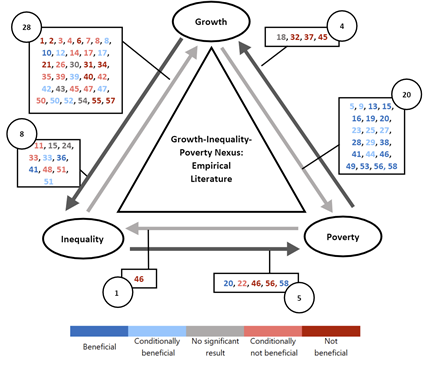
\includegraphics[width=\textwidth]{figure/triangle_relations.png}
    \source{\citet{cetl21}}
    \label{fig:triangle relations}
\end{figure}

경제성장과 불평등의 관계에 대한 연구에서 기회불평등의 개념의 도입은 비교적 최근에 이루어 졌다.
\citet{mnr13, mnr14}는 각각 미국과 전 세계를 대상으로 기회불평등과 경제성장 간의 관계를 연구했는데 노력의 불평등과 경제성장의 관계는 유의하지 않지만, 기회의 불평등과 경제성장 사이에는 분명한 음의 관계가 있음을 발견하였다.
\citet{metl13}은 농경자본을 도구변수로 사용해 교육의 기회불평등을 측정하고, 기회불평등과 경제성장 사이에 음의 관계가 있다고 주장한다.

\citet{mnr13}은 미국의 50개 주를 대상으로 각 주별로 개인 소득의 총불평등을 기회불평등과 노력불평등으로 분해한 패널 자료를 구성하고, 이들 두 변수를 주별 경제성장률과 연결시켰다.
이들은 기회의 불평등과 노력의 불평등이 경제성장에 각각 음과 양의 상반된 영향을 미침을 보임으로써, 선행 연구에서 도출되는 불평등과 경제성장 사이의 모호한 관계가 기회불평등과 노력불평등 각각이 경제성장에 미치는 효과가 서로 상반되기 때문이라고 주장하였다.
\citet{mnr13}의 연구는 불평등과 경제성장 연구의 범위를 확장하면서 불평등이 성장에 미치는 보다 자세한 메커니즘을 분석한다는 점에서 의미 있는 기여를 하고 있다.
그러나 그들은 미국 내의 50개 주를 대상으로 분석하고 있기 때문에, 이 연구로부터 도출된 결과의 해석은 제한적일 수 있다.
첫째, 분석대상인 미국의 주 간에 사람들의 자유로운 이동이 가능하므로 기회의 불평등이 낮은 지역으로 사람들이 이주하는 내생성이 존재할 수 있다.
둘쩨, 경제성장과 불평등간의 관계에서 관심 단위는 주로 국가라는 점에서 한 국가내의 서로 다른 지역을 대상으로 한 연구의 결과를 직접 젹용하기 어렵다.

 \citet{fetl18}는 전세계 42개국에서 117개의 가구조사와 134개의 인구통계학적 건강조사 자료를 취합해 각국의 불평등도를 1985년부터 2005년까지 5년 간격으로 측정하여 소득의 불평등에서 기회의 불평등이 차지하는 비중이 약 5-13 퍼센트라고 보고한다.
 그들의 분석결과에 의하면, 경제성장과 기회의 불평등 사이에는 음의 관계가 나타났지만 그 결과는 그리 강건하지 못하다.
\citet{fetl18}은 \citet{mnr13}에서 도입된 기회불평등과 경제성장간의 관계에 대한 연구를 국가단위로 확장시켰고, 다양한 국가에서 소득 및 건강의 기회불평등을 측정했다는데 의의가 있다.
 또한 불평등이 경제성장에 부정적 영향을 준다는 주장에 대한 반론을 제기하는 최소한의 근거를 제시하였다.
 그러나 그들의 연구에서 사용한 환경에는 기회불평등 문헌에서 중요한 환경 요인으로 간주하는 ‘부모의 능력 변수(부모의 학력, 소득, 재산 등)’가 제외되어 있다.
 
\citet{ane20}는 기회불평등 개념을 경제성장괴 불평등간의 관계에 도입한 가장 최신의 실증연구이다.
이 연구는 총 111개국을 대상으로 하여 불평등의 척도로 각 국가의 소득의 지니계수를 사용하였다.
세대간 소득 또는 교육탄력성을 기회불평등의 척도로 활용하였고, 기회불평등의 정도가 높을 수록 소득불평등이 경제성장에 부정적 영향을 주는 것을 확인하였다. 
\citet{ane20}는 국가간 종단자료를 이용하여 기회불평등과 경제성장 간의 유의미한 부정적 관계를 확인한 연구이다.
그러나 \citet{corak13}의 지적과 같이, 비슷한 수준의 세대간 탄력성이 측정되는 집단들 간에도 기회불평등은 큰 차이가 있을 수 있다.
따라서 이 연구는 기회불평등의 개념을 도입했지만 기회불평등 지수를 사용하지 않았다.


\subsection{기회불평등}

경제학에서 불평등에 관한 연구는 소득, 교육수준, 건강과 같이 인간이 이루는 성취의 불평등에 대하여 그 윈인을 고려한 기회의 불평등(Inequality of Opportunity)으로 그 연구범위가 확장되고 있다.
기회불평등의 개념은 평등주의 철학자들로부터 먼저 연구되었는데, 이들은 한 사회에서 구성원들이 만들어 내는 성취의 불평등이 각 개인의 순수한 의지와 무관한 요소에 의해 발생한다면 이것은 도덕적으로 정당화 할 수 없고, 따라서 사회는 이러한 불평등을 제거하는데 힘써야 한다고 주장한다.
예를 들어, 학생의 학업성취도를 부모의 경제력과 학생 본인의 노력의 함수라고 가정하면, 학업성취도의 총불평등은 부모의 경제력 차이에 기인하는 불평등과 본인 노력의 차이에 기인하는 불평등으로 분해될 수 있다.
이때 부모의 경제력 차이는 환경(혹은 기회) 요인으로서 학생 개인에게 그 책임을 지을 수 없기 때문에, 환경의 차이로부터 발생하는 학업성취도의 불평등은 정당화되기 어렵고 이를 줄이거나 없애기 위해 노력해야 한다.

기회불평등에 대한 본격적인 연구는 \citet{Rawls99}로부터 시작되었다.
 그는 개인의 성취를 노력, 환경, 그리고 운이 복합적으로 작용한 결과라고 말한다.
 그에 의하면 성취의 불평등은 그 원인에 따라 개인에게 책임을 귀속시킬 수 있는 부분과 책임을 귀속시킬 수 없는 부분으로 나뉠 수 있다.
 노력의 차이에 의해 발생하는 불평등에 대해서는 마땅히 그 개인이 책임져야 하겠지만, 개인의 의지와 무관하게 주어지는 환경의 차이에 따른 불평등은 도덕적으로 정당화하기 어렵다.
 
롤즈의 평등사상은 현대적 의미로 개인에게 “동등한 출발선” 또는 “기울어지지 않은 운동장”을 보장해야 한다는 개념으로서, 그는 이러한 “공정한 기회”의 제공을 위하여 실질적인 기회평등이 필요하다고 보았다.
동일한 천부적 능력과 야망을 가진 사람들에게는 그 사람의 가정환경, 상속된 부의 크기, 인종, 성 등과 무관하게 동등한 성취의 전망(prospects of success)이 보장되어야만 한다는 것이다.
\footnote{\citet{Rawls99}, p.63.}

기회평등의 원칙은 드워킨(Ronald Dworkin), 아네슨(Richard Arneson), 코헨(Gerald. A. Cohen) 등의 정치철학자들에 의하여 꾸준히 연구가 진행되었고, \citet{Roemer98}에 이르러 비로소 경제학에 적용가능한 개념으로 정립되었다.
\citet{Roemer98} 이후 많은 경제학 연구들이 기회불평등 개념을 실증분석에 적용하고 있다.
\footnote{기회불평등을 다룬 경제학 연구들은 \citet{rnv12}, \citet{fnp15}, \citet{rnt16}에 잘 정리되어 있다.}
본 연구는 이들 연구에서 성취의 불평등도를 기회의 불평등도과 노력의 불평등도로 분해하는 방법을 차용해 불평등의 두 구성요소 각각이 한 국가의 경제성장에 미치는 영향을 실증적으로 분석한다.

\section{실증분석 방법}

본 연구는 \citet{kno17}의 연구를 자료와 불평등 지수 두 부분에서 확장한다.
자료 측면에서 기존연구가 기회불평등 측정을 위해 사용한 TIMSS 이외에 또 다른 국제교육평가 자료인 PISA를 사용한다. TIMSS만을 사용할 경우 1995년부터 2019년 가운데 총 7개 년도에 대한 기회불평등 측정이 가능하고 그 가운데 경제성장과의 관계를 분석하는데는 최대 6개 년도의 자료를 활용 할 수 있다. PISA를 추가적으로 연구하여 2000년부터 2018년 가운데 5개 년도의 시점에 대한 불평등 측정이 추가되고 특히 2003, 2015년은 두 자료가 모두 생성되에 두 자료의 차이점에 대한 비교 연구 역시 진행할 수 있다.

기회불평등의 측정에 있어 \citet{betl12}에서 제시한 개선점을 활용한다.
교육성취인 시험점수를 기여요인에 따라 환경으로 인한 기회의 불평등과 그 밖의 요인에 의한 잔여불평등으로 구분하여 측정한다.
그후 잔여불평등에서 직접 관찰할 수 없지만 환경의 영향을 받은 요인을 분리하여 노력불평등을 측정한다.

먼저, 기회의 불평등은 대체로 경제성장에 부정적인 영향을 미칠 가능성이 높다.
기회의 불평등이 존재하는 경우, 보다 우월한 노력을 투입한 사람들보다는 우월한 출신배경을 가진 사람들이 인적자본을 축적하기에 유리한 환경이 조성되고, 개인들의 노력이 경제 내에서 적절한 보상을 받지 못할 수 있기 때문이다.
반면, 노력의 불평등은 경제성장에 긍정적인 영향을 미칠 가능성이 높다.
상이한 노력을 투입한 사람들 사이의 소득불평등은 상이한 노력에 대한 보상을 반영하기 때문에, 노력의 불평등은 사람들이 더 많은 노력을 투입할 유인을 제공하기 때문이다.
기존의 실증연구에서 불평등이 경제성장에 미치는 영향이 확정적인 방향으로 도출되지 않는 이유 중 하나는 기회의 불평등과 노력의 불평등 각각이 경제성장에 미치는 효과가 서로 상반되기 때문이다.

본 연구에서는 중학생들의 학업성취도를 이용해 불평등을 측정하기 때문에, 본 연구가 분석하는 불평등의 효과는 엄밀하게는 경제적 불평등의 효과가 아니라 교육성취도의 불평등의 효과이다.
일반적으로 경제적 불평등은 교육성취도의 불평등과 전반적인 경제 구조로부터 발생하는 불평등이 결합되어 있으므로 본 연구에서는 경제적 불평등이 경제성장에 미치는 전체 효과의 일부분만을 분석하고 있다.
이러한 한계점은 여러 국가들을 대상으로 기회불평등과 노력불평등을 측정해야 하는 실증적인 어려움으로부터 발생한다.

본 연구에서는 불평등을 경제성장과 연결시키기 때문에 경제성장을 표현하는 자료들 또한 필요하다.
우리는 선행 연구들을 따라 Penn World Tables(PWT)을 이용해 각 국가의 시점별 1인당 GDP 및 기타 거시자료들을 구축한다.
PWT는 183개국에 대해 1950년부터 2019년까지의 인구, 실질총생산, 물가수준, 고정자본수준 등 방대한 거시자료를 축적한 데이터베이스 이다.
TIMSS와 PISA의 조사대상인 98개국의 거시자료 역시 PWT에 포함되어 있다.

\subsection{불평등지수의 계산}
우리는 \citet{mnr13}의 연구방법을 따라 TIMSS와 PISA의 국가별 각 시점 자료에 대해 아래와 같은 방법을 적용해 학업성취도의 총불평등도과 그것을 분해한 기회불평등도 및 잔여불평등도를 측정한다. 

개인 $i$가 $N$명으로 구성되어 있는 어떤 사회의 한 구성원이라고 가정하자$(i \in \{1,\ldots,N \} )$.
개인 $i$가 속하는 환경변수 $C_{ic}$는 개인의 성취에 영향을 주면서 그 개인이 스스로의 의지로 선택할 수 없는 요인이다.
환경변수는 부모의 학력, 출생지의 규모, 부모의 소득, 인종, 성별 등 실제 자료에서 쉽게 관찰할 수 있는 다양한 요소가 될 수 있다.
개인 $i$가 속하는 환경 $C_i$는 이러한 환경변수$C_{ic}$ 들의 c-터플(c-turple) $C_i = \{C_{1i}, \ldots , C_{ci}\}$이다. 
환경유형 $T= \{1, \ldots , t \}$, $t= ||C_1|| \times \cdots \times ||C_c||$는 편의를 위하여 가능한 환경의 집합 $\{ C_i \}$을 정의역으로 취하는 지표(index)이다.

개인의 학업성취도를 $y_i$, 개인이 속한 환경유형을 $T_i$, 개인이 하는 노력을 $e_i$라고 표시하자.
기회불평등의 관점에서 성취는 개인이 속한 환경 및 환경과 무관한 개인의 노력의 결과라고 정의한다.
이때 성취 $y_i$의 확률밀도함수 $f(\cdot)$는 $ y_i = f(T_i, e_i)$와 같이 표시할 수 있다.

본 연구에서 계산하는 기회불평등 지수는 \citet{fng11}에서 제시한 방법에서 출발한다.
타일-0 지수(Theil-0 index)는 지니계수 이외의 방식으로 불평등 정도를 측정하는 대표적인 지수이다. (이 지수는 대수 평균 편차(mean log deviation) 라고도  불린다.) 
한 국가의 모든 학생의 성적을 $Y= (y_1, \ldots , y_n)$ 이라고 할 때 타일-0 지수의 식은 다음과 같다.
\begin{equation}
\label{eq:theil0}
 T(Y)=\frac{1}{N} \sum_{i=1}^{N} \ln \left(\frac{\bar{y}}{y_{i}}\right)
\end{equation} 
위 식에서 $\bar{y}$는 성적의 평균값이다.
따라서 모든 학생이 동일한 성적을 얻는 완전 평등한 상태일 경우 지수의 값은 0이 되고 학생간 성적의 차이가 클수록 그 값이 커진다.
일반적인 불평등 연구에서는 지니계수가 불평등 지표로서 주로 사용하지만, 지니계수는 가산적 분해가능성(additively decomposibility)이 없기 때문에 총불평등을 윈인에 따라 나눠 분석하는 기회불평등 연구에서는 한계가 있다.
반면에 타일-0 지수를 이용해 측정한 불평등은 간단하게 기회불평등과 노력불평등으로 분해된다.

우리는 아래의 식 (\ref{eq:theil0-decompose})을 통해 성적의 총불평등도를 기회불평등도와 노력불평등도로 분해한다.
\begin{equation}
T(v)=T(\bar{v})+\sum_{t=1}^{T} p_{t} T\left(v^{t}\right)
 \label{eq:theil0-decompose}
\end{equation}
이 식에서 $T(v)$는 총불평등 지수, 즉 학생들의 원 성적을 이용해 계산한 타일-0 지수의 값이다.
$T(\bar{v})$은 동일한 환경에 속한 학생들의 성적이 그 환경의 평균 성적($\bar{v}$)으로 모두 같다고 가정했을 때 도출되는 불평등지수의 값이다.
따라서 $T(\bar{v})$로 측정되는 불평등은 상이한 환경에 의한 차이만을 반영하기 때문에 기회의 불평등도로 간주한다.
$p_t$은 환경유형이 $t$인 학생의 비율이고 $T(v^t)$는 환경유형이 $t$인 학생들에서 해당 환경유형의 평균성적 $\mu _t$을 차감한 성적을 이용한 불평등지수의 값이다.
 타일-0 지수의 경우 식 (\ref{eq:theil0-decompose})이 항상 성립하기 때문에, $T(v) - T(\bar{v})$는 엄밀하게는 노력의 불평등도라기 보다는 총불평등에서 기회불평등을 제외한 잔여(residual) 불평등도이다.
 
%타일-0 지수의 가산적 분해가능성에 의해 식 (\ref{eq:theil0})은 다음과 같이 분해할 수 있다.
%\begin{equation}
 %\label{eq:theil0-decompose}
 %T(Y)=T(C ' \cdot \beta) + T(\epsilon)
%\end{equation}
%이 식에서 $T(Y)$는 총불평등 지수, 즉 학생들의 원 성적을 이용해 계산한 타일-0 지수의 값이다.
 %$T(C ' \cdot \beta)$은 학생들의 성적 가운데 환경에 의한 부분에 대한 불평등지수의 값으로서 기회의 불평등도를 의미하고,  $T\left(\epsilon\right)$는 잔여(residual)불평등도 이다. 

위에서 정의한 환경 $C$가 성적에 영향을 미치는 모든 환경변수들을 포괄하고 있다면, $T(\bar(v)$는 정확하게 기회의 불평등도를 표현하고, $T(v) - T(\bar{v})$는 노력의 불평등도를 표현할 것이다.
그러나 관측되는 환경은 기회의 불평등에 영향을 미치는 전체 환경들의 부분 집합에 불과하다.
예를들어 지능이나 부모의 소득수준은 학생의 성적에 중요한 요소이지만 본 연구의 자료에서 조사되기 않았기에 잔여불평등에는 관찰하지 못한 환경의 영향이 존재한다. 
또한 유전병과 같이 환경으로 생각할 수 있는 다른 요인과 운(luck) 마저도 결과에 영향을 주지 못한다.
그러므로 $T(\bar(v))$는 기회의 불평등도의 하한을 표현하고, $T(v) - T(\bar{v})$는 기회의 불평등과 노력의 불평등이 혼합되어 있는 잔여불평등도를 표현한다.
결과적으로 $T(\bar{v})$는 기회불평들을 매우 엄격하게 측정하고 있다고 볼 수 있다.
 
\citet{betl12}은 앞서 계산된 불평등지수의 잔여불평등 부분에 대하여 \citeauthor{Roemer98}의 순수한 노력(pure effort) 개념을 적용한 개선 방법을 제안한다.
 \citet{Roemer98}는 개인의 성취는 그 개인이 속한 환경과 스스로의 노력 두 요소의 결과라고 이야기 한다.
이때 노력은 환경에 전혀 영향을 받지 않는다는 의미에서 순수한 노력이어야 한다.
문제는 현실에서 관찰하는 대부분의 노력과 관련된 정보가 환경의 영향을 받는다는데 있다.
예를들어 높은 시험점수를 받는데 있어 노력의 변수로 학생의 공부시간을 생각할 수 있다.
하지만, 과외 또는 학원과 같은 사교육에 들이는 공부시간을 제외한 순수한 자습시간 만을 살펴봐도 좋은 교육환경에 속한 학생들이 더 많은 자습시간을 보장받는다.\footnote{\citet{ohetl16}}

\citet{betl12}은 노력의 불평등을 포함하는 잔여불평등의 기반이 되는 $T(v^t)$에서 상이한 환경에 의해 얻게되는 성적을 정제하여 이를 기회불평등의 계산에 반영할 것을 제안한다. 
구체적인 방법은 다음과 같다.
식 (\ref{eq:theil0-decompose})에서 기회불평등을 계산하기 위해 개별환경의 평균성적을 계산했다.
환경별 평균성적은 모수적 추정에 의하면 환경조건부 성취의 기댓값 $E[Y |C]$와 같다.
앞서 개인의 성취 $y_i$는 개인이 속한 환경 $C_i$와 개인이 들인 환경과 무관한 노력 $e_i$의 함수라고 정의하였다.
편의를 위해 위 함수관계가 선형이라고 가정하면 아래의 식과 같다.

\begin{equation}
\label{eq:ols}
\begin{aligned}
    y_{i} & = E[Y|C_i] + \epsilon _i \\
        &=\beta _0 +  \beta _1 C_{1,i} + \cdots + \beta _c C_{c,i} + \epsilon _i 
\end{aligned} 
\end{equation}

잔차 $\epsilon _i$는 노력 $e_i$ 이외에 환경 $C_i$의 영향을 받는 부분이 포함되고 따라서 환경별로 잔차의 분포는 상이할 것이다.
\citeauthor{betl12}는 이를 계량경제학의 관점에서 선형회귀모형의 오차항에 이분산성(heteroscedasticity)이 있다는 것으로 생각했다.
다시말해 잔차의 환경조건부 분산 $\sigma ^2 _c = Var[\epsilon |C_c]$이 환경별로 상이하다는 것이다.
이러한 이분산성을 해소하고 그 과정에서 잔차에 존재하는 환경의 영향을 받는 성취를 분리해 낸다면 \citet{fng11}에서 제시하는 엄격한 기준보다 좀 더 완화된 기회불평등 정도를 측정할 수 있을 것이다.

잔차 $\epsilon$에 존재하는 환경의 영향을 받는 성적은 다음의 과정으로 분해한다.
잔차의 총분산 $\sigma ^2$은 개별 환경유형의 잔차의 분산 $\sigma _c^2$과 그 유형의 밀도 $f_c$의 곱의 합 $\sigma ^2 =  \sum _c f_c \sigma ^2 _c$으로 표현할 수 있다. 
이를 엄밀히 표현하면 다음과 같다.
\begin{equation}
\label{eq:bjork}
 \begin{aligned} y_{i} &= \beta _0 +  \beta _1 C_{1,i} + \cdots + \beta _c C_{c,i} + \epsilon_{i} \\ &= \beta _0 +  \beta _1 C_{1,i} + \cdots + \beta _c C_{c,i} +\epsilon_{i}-\underbrace{\epsilon_{i} / k \sigma_{c}}_{u_{i}}+\underbrace{\epsilon_{i} / k \sigma_{c}}_{u_{i}} \\ &= \beta _0 +  \beta _1 C_{1,i} + \cdots + \beta _c C_{c,i} +\widetilde{\epsilon}_{i}+u_{i}, \end{aligned}
\end{equation}
이때 $k = ( 1 / \sum _c f _c \sigma ^2 _c ) ^{-1/2}$이다.
식 (\ref{eq:bjork}) 마지막 줄은 세 부분으로 구분되는데 $\beta _0 +  \beta _1 C_{1,i} + \cdots + \beta _c C_{c,i}$는 환경의 영향을 받는 성취이다. 따라서 $C'\hat{\beta}$는 환경별 평균성취가 된다. $\widetilde{\epsilon}_{i}$는 잔차에 존재하는 개인별 성취에 대한 환경의 기여분이다. $u_i$는 성취에 대한 개선된 잔여 기여분이다.
따라서 타일-0 지수를 이용한 기회불평등과 잔여불평등을 구하는 식 (\ref{eq:theil0-decompose})는 아래와 같이 바뀐다.
\begin{equation}
 \label{eq:theil0-bjork}  
  T(v)=T(\bar{v}+\widetilde{\epsilon}_i)+ \sum_{t=1}^{T} p_{t} T\left(v^{t}-\widetilde{\epsilon}_i\right)
\end{equation}
우변의 첫번째 항인 $T(\bar{v}+\widetilde{\epsilon}_i)$는 환경별 평균성취와 환경의 영향을 받는 개인별의 성취의 합에 대한 불평등으로 기회불평등을 나타낸다.
따라서 $T(v) - T(\bar{v}+\widetilde{\epsilon}_i)$는 새로운 잔여 불평등이 된다.

\subsection{자료에 대한 기초 분석}

먼저 각 국가의 시점별 불평등을 측정하기 위해 우리는 전 세계 중등학생들의 학업성취도를 국제적으로 측정하는 TIMSS와 PISA의 자료를 사용한다.
TIMSS는 국제 교육성취도 평가협회(International Association for the Evaluation of Educational Achievement, IEA)의 주관 하에 시행되는 국제 학업성취도 평가이다.
TIMSS는 1995년부터 매 4년마다 약 50여개 국가에 거주하는 4학년(초등학교 4학년)과 8학년(중학교 2학년) 학생들을 대상으로 수학과 과학 두 과목에 대해 동일한 시험을 실시하여 학생들의 학업성취도를 측정한다.
PISA는 경제개발협력기구(Organisation for Economic Co-operation and Development, OECD)의 주관 하에 시행되는 국제 학업성취도 평가이다.
PISA는 만 15세 학생의 읽기, 수학, 과학 소양의 성취와 추이를 국제적으로 비교하고, 교육맥락변인과 성취 사이의 관계를 파악하기 위해 2000년부터 3년을 주기로 시행되는 국제 비교 연구이다.
 
TIMSS와 PISA 자료는 자료의 질적 측면에서 장점을 가지고 있다.
두 자료는 학생들의 학력 점수와 더불어  학생, 학교, 교사, 학부모에 대한 교육환경 자료를 수집하므로 기회불평등 연구에서 핵심적인 학생의 환경에 대한 정보가 존재한다.
각 우리는 모든 조사연도에 걸쳐 총 98여 개국 학생들의 학업성취도 및 가족배경 자료를 이용할 수 있다.
소득이나 재산을 통해 경제적 불평등을 측정하는 연구는 개별 국가의 서로 다른 기관에서 작성하는 이질적인 자료들을 바탕으로 불평등도를 측정하기 때문에 측정기준과 시점이 서로 상이하고 따라서 자료의 질이 상이한 문제가 존재한다.
이들 자료는 매년 동일한 기관에서 각 주기마다 동일한 시험문제와 설문조사 문항들을 이용해 자료를 구축하기 때문에 자료의 균질성이 매우 높다고 평가할 수 있다.

하지만 두 자료는 국제교육평가라는 공통점에도 불구하고 동일한 맥락에서 분석할 수 없는 차이점을 가진다.
먼저 두 조사의 응답자의 차이에 의한 응답률의 차이가 상당하여 분석에 주의를 요한다. 두 자료 모두 설문지는 크게 학생, 학교, 교사 그리고 가정환경의 넷으로 구분할 수 있다. PISA의 경우 응답자가 학생, 학부모, 교사 및 교육행정가(교장 등)로서 대부분의 항목에서 응답이 잘 이뤄지고 있다. 반면 TIMSS는 응답자가 학생, 교사 및 교육행정가로 제한되어 학생이 가정환경을 응답해야 하므로 부모의 학력이나 가정의 소유재산 등 본 연구에서 활용하려는 환경변수에 대한 응답률이 제한적일 수 있다.

\begin{table}[htbp]\centering
\def\sym#1{\ifmmode^{#1}\else\(^{#1}\)\fi}
\caption{자료별 응답률 \label{tab:pnt_response}}
\begin{tabular}{c|ccccc} 
자료 & 관측수 & 평균 & 표준편차 & 최솟값 & 최댓값 \\
\hline PISA & 407 & $.9529165$ & $.0450238$ & $.3573059$ & $.9982405$ \\
TIMSS & 276 & $.7804372$ & $.1274786$ & $.3429133$ & $.9920338$
\end{tabular}
\end{table}

표 (\ref{tab:pnt_response})는 본 연구에서 활용하는 환경변수들에 대한 국가별 응답률에 대한 요약통계량 이다. PISA의 경우 극단치인 1개 관측치를 제외하고 대부분의 경우 90\%이상의 응답률을 보인 반면 TIMSS의 경우 응답률이 50\%이하인 경우가 총 276개 자료 가운데 12건 존재하였다. 
TIMSS에서 나타나는 환경변수의 낮은 응답률이 의도하지 않았더라도 대체로 열악한 환경에 속한 학생들이 응답하지 않았을 가능성이 존재한다.
따라서 TIMSS를 바탕으로 하는 기회불평등 지수의 과소측정 가능성이 존재한다.

다음으로, 두 자료가 측정하려는 교육성취가 상이하다는 점을 고려해야 한다.
TIMSS의 측정 대상인 교육성취는 학생이 교과과정에서 배운 내용을 얼마나 잘 알고 있는가인 반면, PISA가 측정하는 교육성취는 학생의 해당 교과목에 대한 문해력(literracy)의 측정에 촛점을 맞춘다.
이들 학업성취도와 문해력이 밀접한 관련이 있음에도 상이한 능력임은 주지의 사실이다.
TIMSS와 PISA에 대한 비교연구인 \citet{wu09}, \citet{Klieme16}는 각각의 자료에서 측정한 국가별 평균점수를 이용하여 학업성취도와 문해력간에 매우 밀접한 관계가 있음을 보였다.
하지만 학업성취도의 경우 교육과정에서 학습한 내용일수록 성취가 높을 수 밖에 없다는 점에서 교육제도가 잘 갖춰진 국가들이 높은 평균점을 받을 가능성이 크다는 점에서 문해력과 큰 차이를 보인다고 주장한다. 
이와같은 결과는 평균성적 뿐만 아니라 본연구의 주제인 교육 불평등에서도 드러나고 있다.
그림 (\ref{fig:bar_pntcompare})은 TIMSS와 PISA가 동시에 치뤄진 2003년과 2015년에 각각의 조사에 참여한 국가들의 교육불평등지수의 평균을 보여주고 있다.
2003년과 2015년 모두 (교육)제도가 잘 갖춰졌을 것으로 생각되는 OECD 국가의 교육불평등이 비OECD 국가들 보다 낮다.
특히 TIMSS로 측정한 학업성취도의 경우 OECD국가의 평균 교육불평등도가 비OECD 국가의 절반수준에 머물렀다.
반면 PISA를 통해 측정한 문해력은 OECD국가의 평균 교육불평등도가 비OECD 국가의 70\% 수준에 달해 학업성취도의 불평등보다 그 격차가 적은 것으로 나타났다.

\begin{figure}
    \centering
    \caption{PISA와 TIMSS 불평등 비교}
    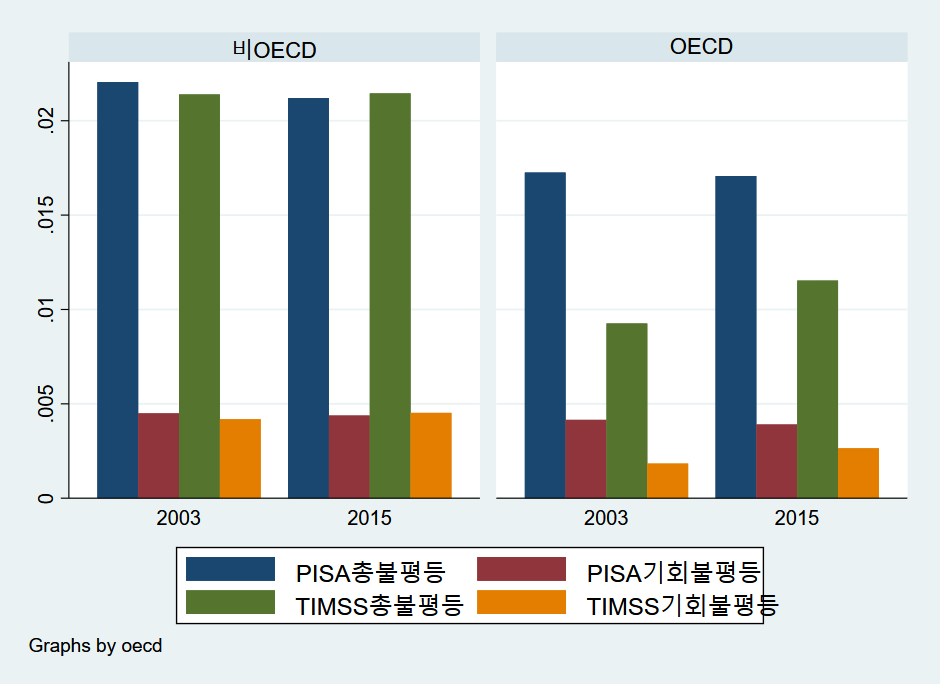
\includegraphics[width=\textwidth]{figure/bar_pntcompare.png}
    \label{fig:bar_pntcompare}
\end{figure}

본 연구에서는 TIMSS의 8학년 학생과 PISA의 학생들에 대한 학업성취도의 총불평등도, 기회불평등도 및 잔여불평등도를 계산한다.
\footnote{정확한 불평등도의 수치와 자료의 기초통계량은 부록에서 제시한다.}
국가별로 학생의 성적을 환경에 대하여 단순선형회귀 하여 환경에 의한 점수와 잔여분에 의한 점수의 추정치를 계산한다. 
여기에 앞서 소개한 \citet{betl12}의 이분산 교정을 이용하여 관측되지 않는 환경에 의한 점수의 추정치를 계산한다.
이 과정에서 환경유형별 오차항의 분산을 추정해야 하기 때문에 특정 유형에 너무 적은 학생이 있을 추정오차가 커지는 문제가 발생한다.
이를 방지하기 위해 환경유형별로 4명 이하의 학생이 존재하는 경우는 분석에서 제외한다.

우리는 두 교육자료에서 제공하는 학생의 수학점수(1st plausible value)를 학생의 학업성취도 성과로서 정의한다.
두 자료는 교육성취를 측정하기 위하여 학생들에게 여러문항의 문제를 제시한다.
각 문항의 점수는 채점이후 문항 반응 이론(item response theory)에 의해 사후적으로 정해지는데 모든 응시생의 평균이 500이고 표준편차가 100으로 조정된 점수가 부여된다.
과목은 수학만을 선정한다. 수학 이외에도 TIMSS는 과학 그리고 PISA는 언어 및 과학 과목의 시험을 더 치른다. 과학과목 역시 두 조사 모두 시행하고 있지만, 과목의 특성상 그 범위가 넓고 실험실의 유무와 같은 국가별 교육환경에 더 영향을 받을 것이다. 이와 같은 영향을 최소화 하기위해 수학과목만을 측정한다. 
 
본 연구에서 환경은 부모의 학력, 가구의 소유물 그리고 가구가 보유한 도서의 수를 이용하여 정의한다.
TIMSS와 PISA 각 자료는 조사시점마다 부친과 모친(또는 남성 및 여성 주 양육자)의 학력을 무학에서 대학원까지 6-7개의 범주형 변수로 제공한다.
우리는 두 개의 학력변수를 단순합 하여 2-12(또는 14)의 항목을 갖는 부모의 학력 변수를 생성한다.
두번째 환경변수는 가구의 소유물 이다.
TIMSS는 매 조사마다 학생의 책상, 방, 인터넷, 컴퓨터 등 네 가지 물건에 대한 소유여부를 조사한다.
PISA의 경우 최대 13가지의 소유물 변수가 존재하지만 자료간 동일성을 유지하기 위해 TIMSS와 유사한 설문 조항 넷을 선택하였다.
모든 소유물 변수는 가변수(Dummy variable) 형태로 값을 취하는데 이를 단순 합하여 0-4의 점수를 가지는 가구 소유물 환경변수를 생성하였다.
마지막으로 장서수는 학생이 속한 가구가 가진 책의 숫자를 10권 미만부터 200권 이상까지 총 1-5의 항목을 가지는 범주형 변수이다.
이상의 세 환경변수에 의한 환경유형은 최대 $13 \times 5 \times 5 = 325$가지 이다.
\footnote{국가에 따라 특정 유형에 한 명도 나오지 않는 경우도 있다.
    예를 들어, 대한민국에서 부모가 모두 대학원졸업 이면서 소유물의 갯수가 0개이고 장서수가 10권 미만인 학생은 없다.} 

\begin{figure}
    \centering
    \caption{1인당GDP와 교육의 총불평등; TIMSS}
    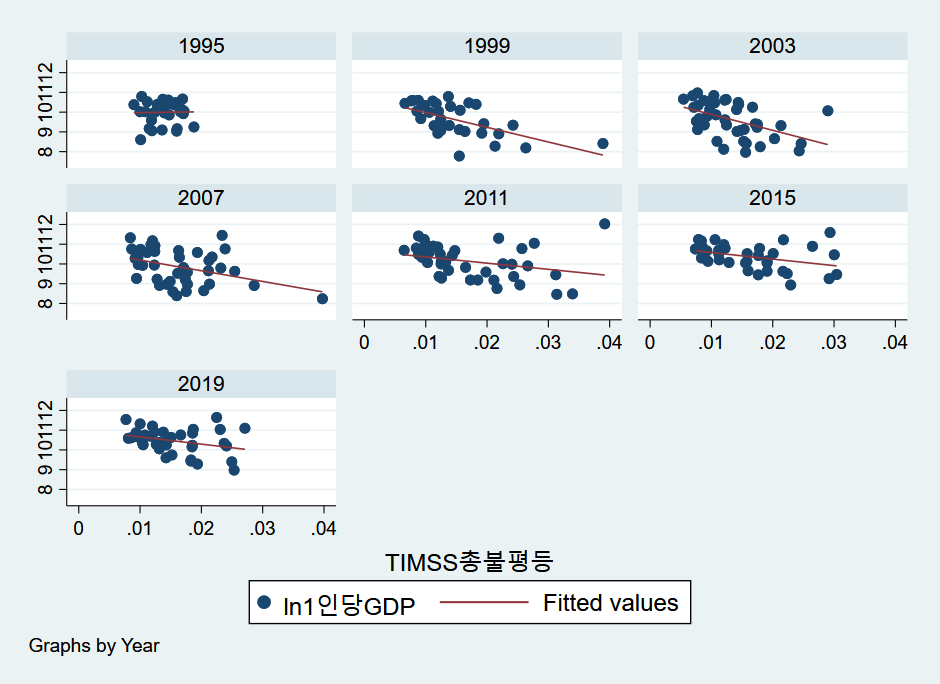
\includegraphics[width=\textwidth]{figure/scatter_lnpcgdp_totmath_timss.png}
    \label{fig:scatter_timss_lnpcgdp_bjtmath}
\end{figure}
그림 (\ref{fig:scatter_timss_lnpcgdp_bjtmath})는 TIMSS 자료상의 국가들의 총불평등과 1인당 국내총생산의 로그값의 관계를 산포도(scatter plot)로 나타낸 것이다.
실선은 각 점들에 대한 맞춤값(fitted value)를 나타냈는데 1995년을 제외한 2000년부터 2019년까지 조사에서 그 값이 모두 우하향 하여 국가의 경제수준과 교육불평등 간에 음의 관계가 있음을 알 수 있다. 

\begin{figure}
    \centering
    \caption{1인당GDP와 교육의 총불평등; OECD vs. 비OECD, TIMSS}
    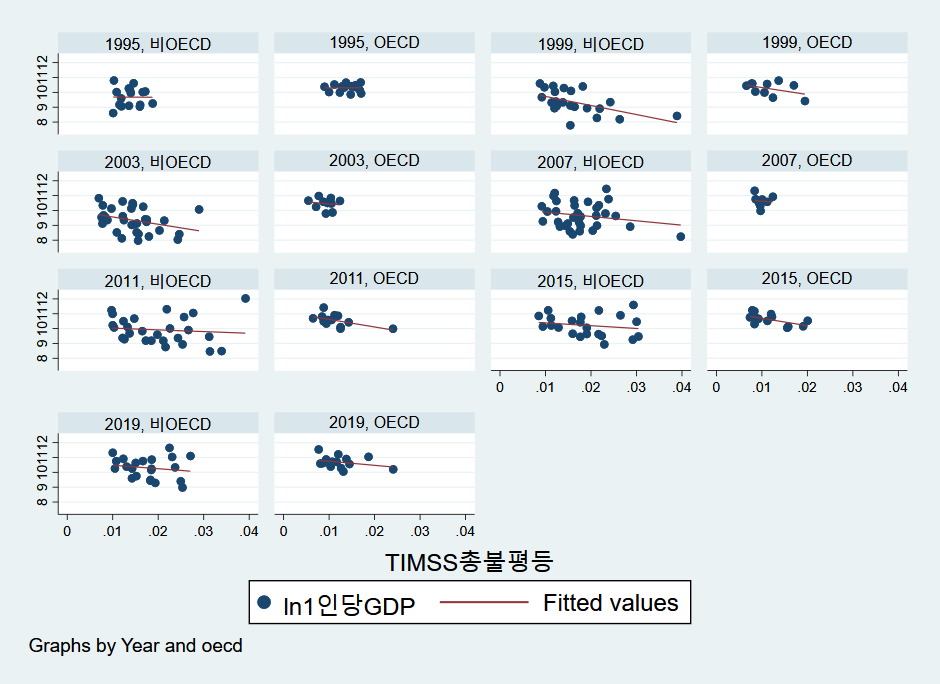
\includegraphics[width=\textwidth]{figure/scatter_lnpcgdp_totmath_timss_oecd.png}
    \label{fig:scatter_timss_lnpcgdp_bjtmath_oecd}
\end{figure}

그림 (\ref{fig:scatter_timss_lnpcgdp_bjtmath_oecd})는 그림 (\ref{fig:scatter_timss_lnpcgdp_bjtmath})을 정보를 OECD 가입국가와 미가입 국가로 나누어 표시하였다.
\footnote{2021년 현재 가입국가는 총 38개국이다. 한국은 1996년 가입하여 TIMSS 1995년을 제외한 나머지 자료에서 OECD 국가로 분류된다. 자세한 가입년도 및 현황은 https://www.oecd.org/about/members-and-partners/ 를 참고하면 된다.}
가장 눈에 띄는 점은 점들의 퍼짐인데, OECD 국가들의 경우 점들이 잘 모여있어 국가별 교육불평등의 정도가 크게 다르지 않음을 알 수 있다. 반면 비OECD 국가의 경우 국가별 1인당 GDP나 교육불형등 수준이 매우 상이함을 알 수 있다.

\begin{figure}
    \centering
    \caption{1인당GDP와 교육의 총불평등; PISA}
    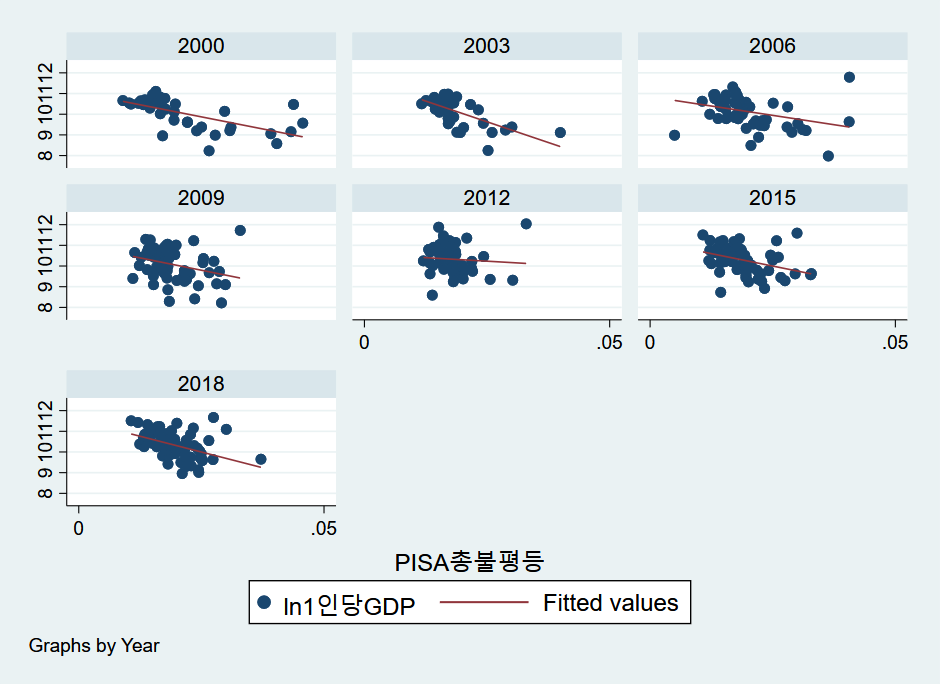
\includegraphics[width=\textwidth]{figure/scatter_lnpcgdp_totmath_pisa.png}
    \label{fig:scatter_pisa_lnpcgdp_bjtmath}
\end{figure}
그림 (\ref{fig:scatter_pisa_lnpcgdp_bjtmath})는 그림 (\ref{fig:scatter_timss_lnpcgdp_bjtmath})와 유사하게 PISA 자료상의 국가들의 총불평등과 1인당 국내총생산의 로그값의 관계를 산포도(scatter plot)로 나타낸 것이다.
2000년부터 2018년까지 조사에서 맞춤값이 모두 우하향 하여 국가의 경제수준과 교육불평등 간에 음의 관계가 있음을 알 수 있다. 

\begin{figure}
    \centering
    \caption{1인당GDP와 교육의 총불평등; OECD vs. 비OECD, PISA}
    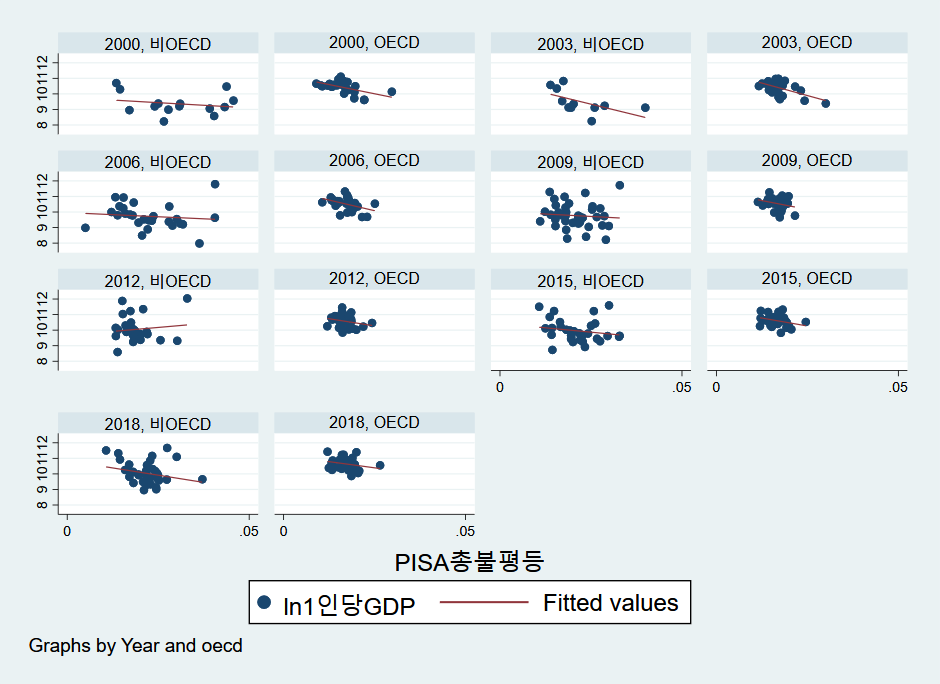
\includegraphics[width=\textwidth]{figure/scatter_lnpcgdp_totmath_pisa_oecd.png}
    \label{fig:scatter_pisa_lnpcgdp_bjtmath_oecd}
\end{figure}

그림 (\ref{fig:scatter_pisa_lnpcgdp_bjtmath_oecd})은 그림 (\ref{fig:scatter_pisa_lnpcgdp_bjtmath})의 내용을 앞서와 마찬가지로 OECD 국가와 비OECD 국가로 나누어 나타낸 것이다.
2012년 비OECD 국가들의 경우 예외적으로 맞춤값이 우상향 하는 것으로 나타나지만 가장 우상단의 극단치인 카타르를 제외한다면 전체적으로 우하향 하는 것으로 볼 수 있다.
 OECD국가들의 점들이 비OECD 국가들에 비해 조밀한 점은 앞서 TIMSS의 경우와 동일하다.
 
\begin{figure}[htpb]
    \centering
    \caption{PISA 총불평등}
    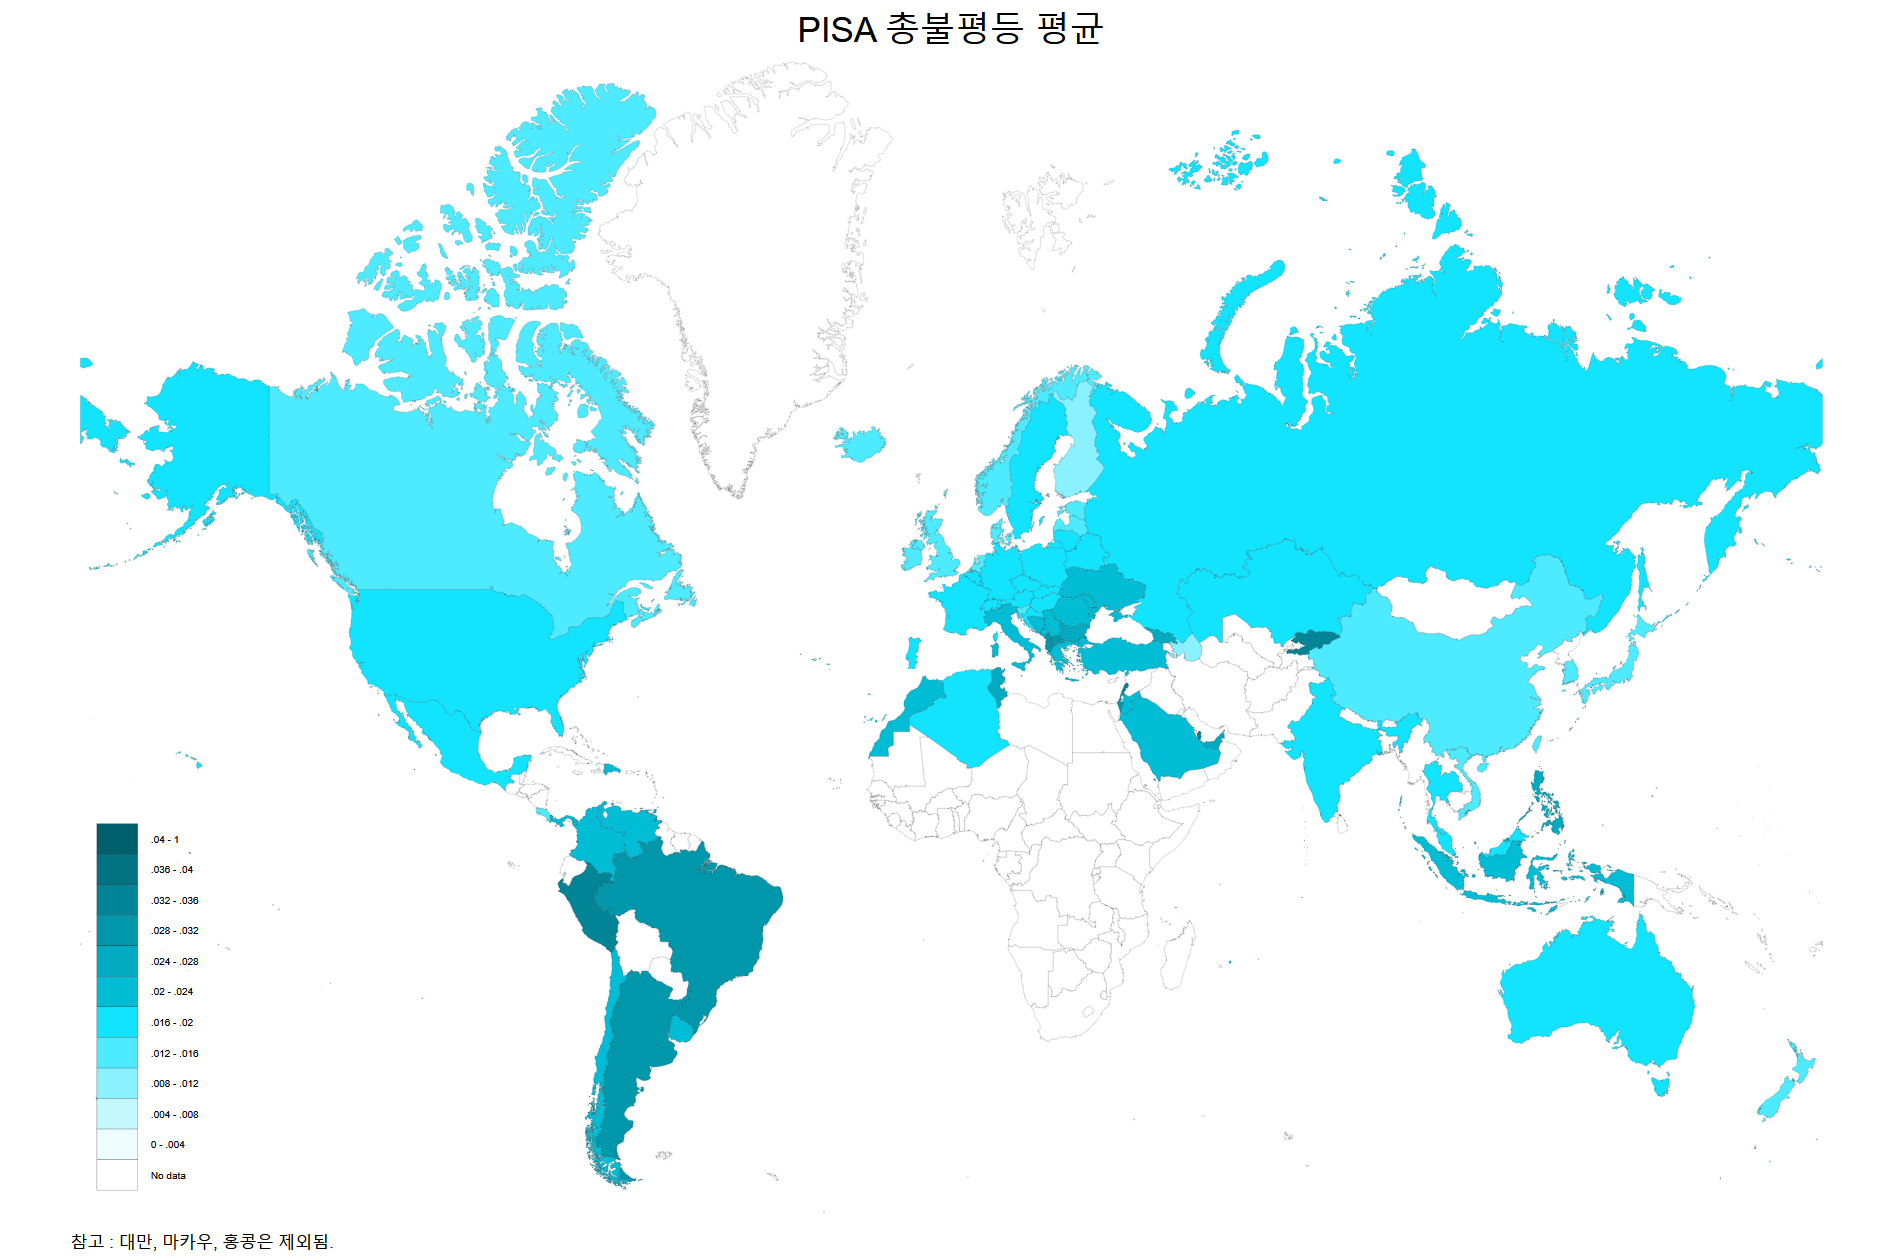
\includegraphics[width=\textwidth]{figure/map_bjtpisa_mean.png}
    \label{fig:map_bjtpisa_mean}
\end{figure}

그림 (\ref{fig:map_bjtpisa_mean})은 PISA 자료를 이용해 측정한 전세계 교육불평등 정도를 2000년 부터 2018년 까지의 평균으로 나타낸 지도이다.
동유럽, 동남아시아, 남아메리카 및 아프리카와 같은 개도국이 많은 지역에서 교육의 총불평등이 높은 것을 확인할 수 있다.
이는 국가의 발전 정도에 맞춰서 발전된 교육제도가 학생들의 교육격차를 줄이는 역할을 하고 있음을 보여준다.

\begin{figure}[htpb]
    \centering
    \caption{PISA 기회불평등의 비중}
    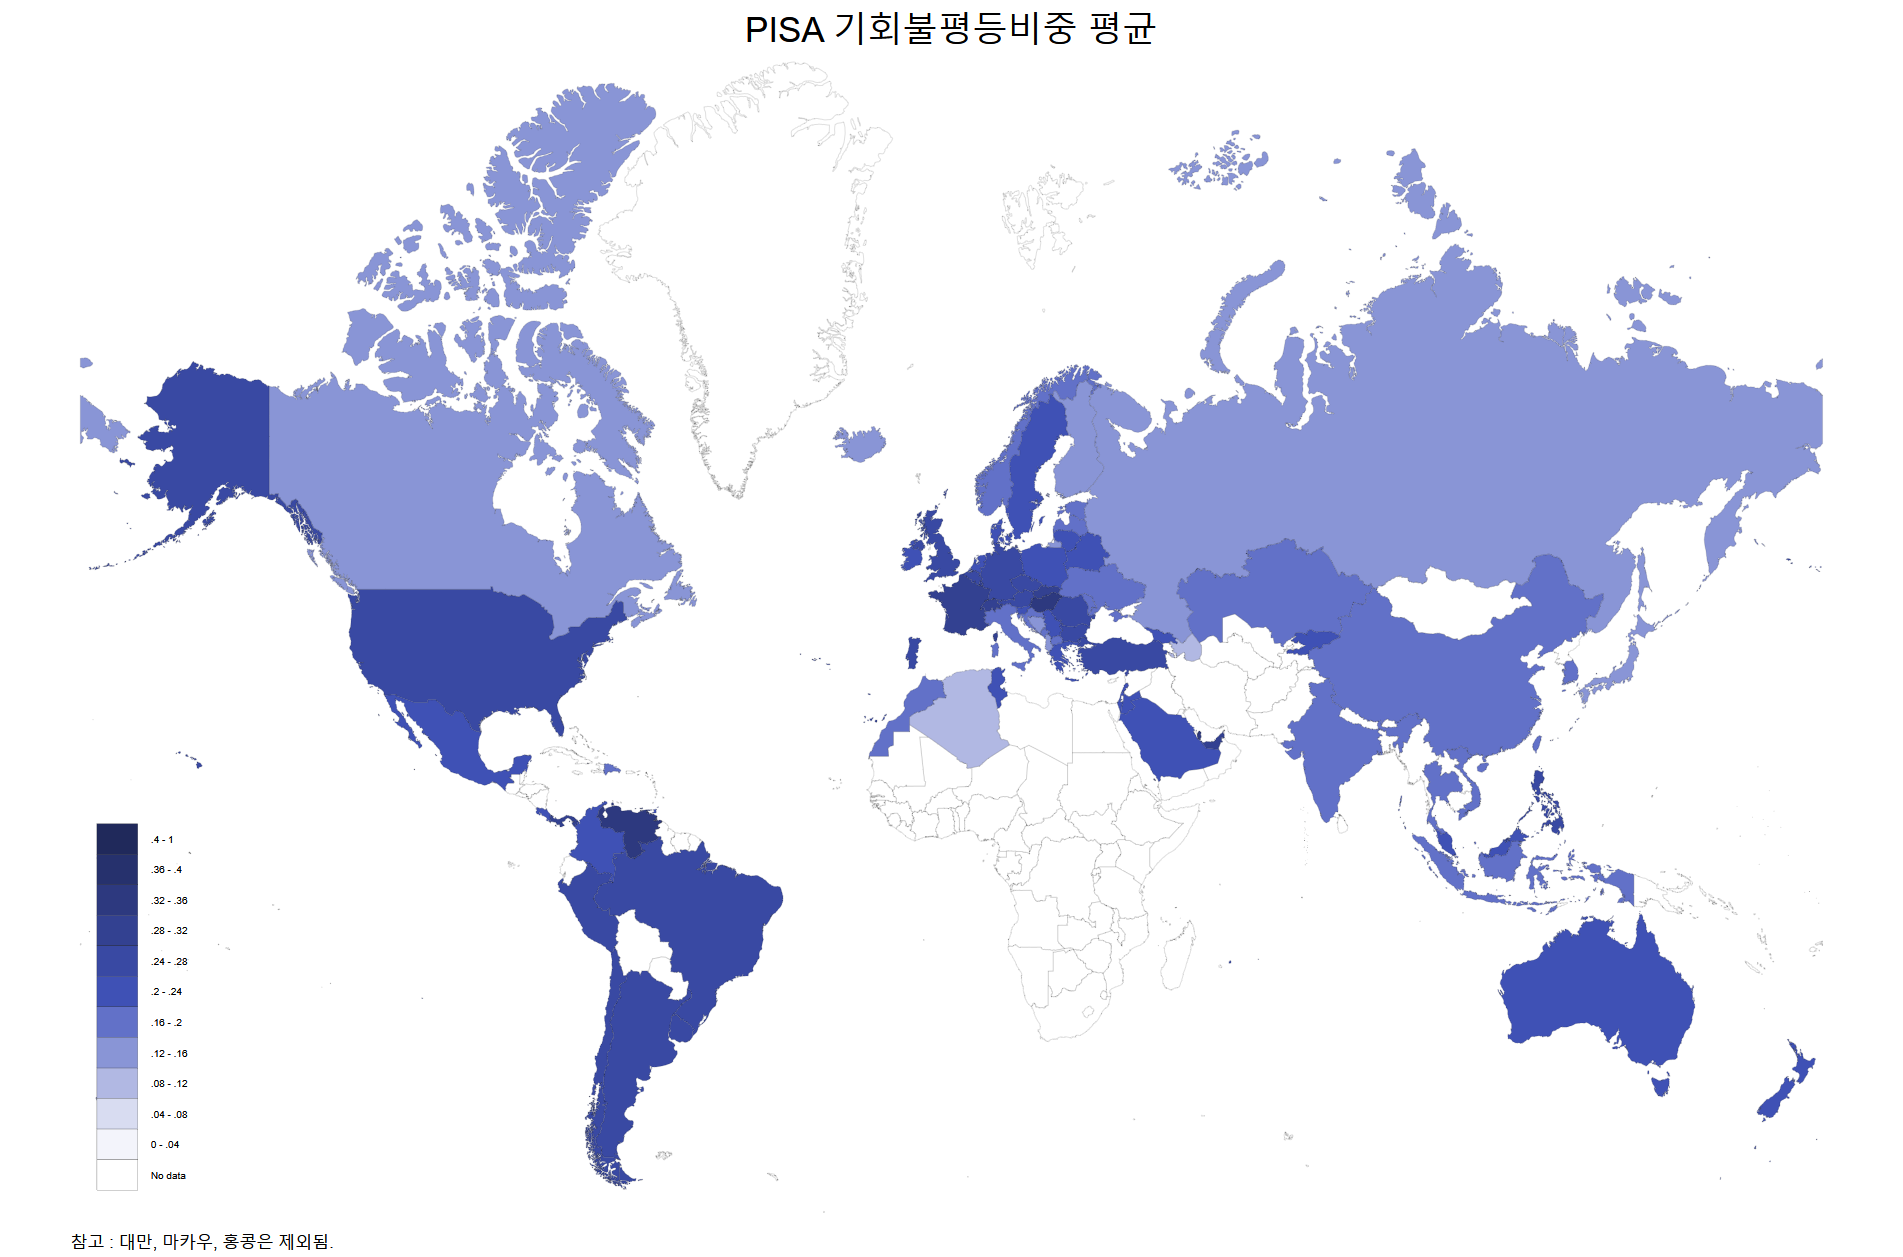
\includegraphics[width=\textwidth]{figure/map_bjrpisa_mean.png}
    \label{fig:map_bjrpisa_mean}
\end{figure}

그림 (\ref{fig:map_bjrpisa_mean})은 그림 (\ref{fig:map_bjtpisa_mean})에서 표시된 총불평등 중에서 기회불평등의 비중이 얼마나 되는가를 나타낸 것이다.
흥미로운 점은 교육의 총불평등이 비교적 낮았던 미국, 서유럽 등의 선진국 지역에서도 기회불평등의 비중은 개도국지역과 비슷하거나 오히려 높은 수준인 것으로 나타났다는 점이다.
선진국의 교육제도가 학생들의 교육격차를 줄이는데 촛점을 맞추고 있다면, 개별 가구에서는 오히려 학생이 좋은 성적을 얻기위한 경쟁에 상당한 영향력을 행사하고 있음을 짐작하게 한다.


그림 (\ref{fig:map_bjrtimss_mean})은 그림 (\ref{fig:map_bjttimss_mean}) 앞선 그림들와 유사하게 TIMSS로 측정한 수학 학업성취도의 총불평등과 총불평등에서 기회불평등의 비중을 1995년 부터 2019년까지 평균값으로 표시한 세계 지도 이다.
TIMSS로 측정한 학업성취도의 경우도 PISA로 측정한 문해도와 마찬가지로 아프리카와 같은 개도국 지역에서 교육의 총불평등도가 높은 반면, 기회불평등의 비중은 서유럽과 같은 선진국에서도 매우 높은 수준임을 확인할 수 있다.

\begin{figure}[htpb]
    \centering
    \caption{TIMSS 총불평등}
    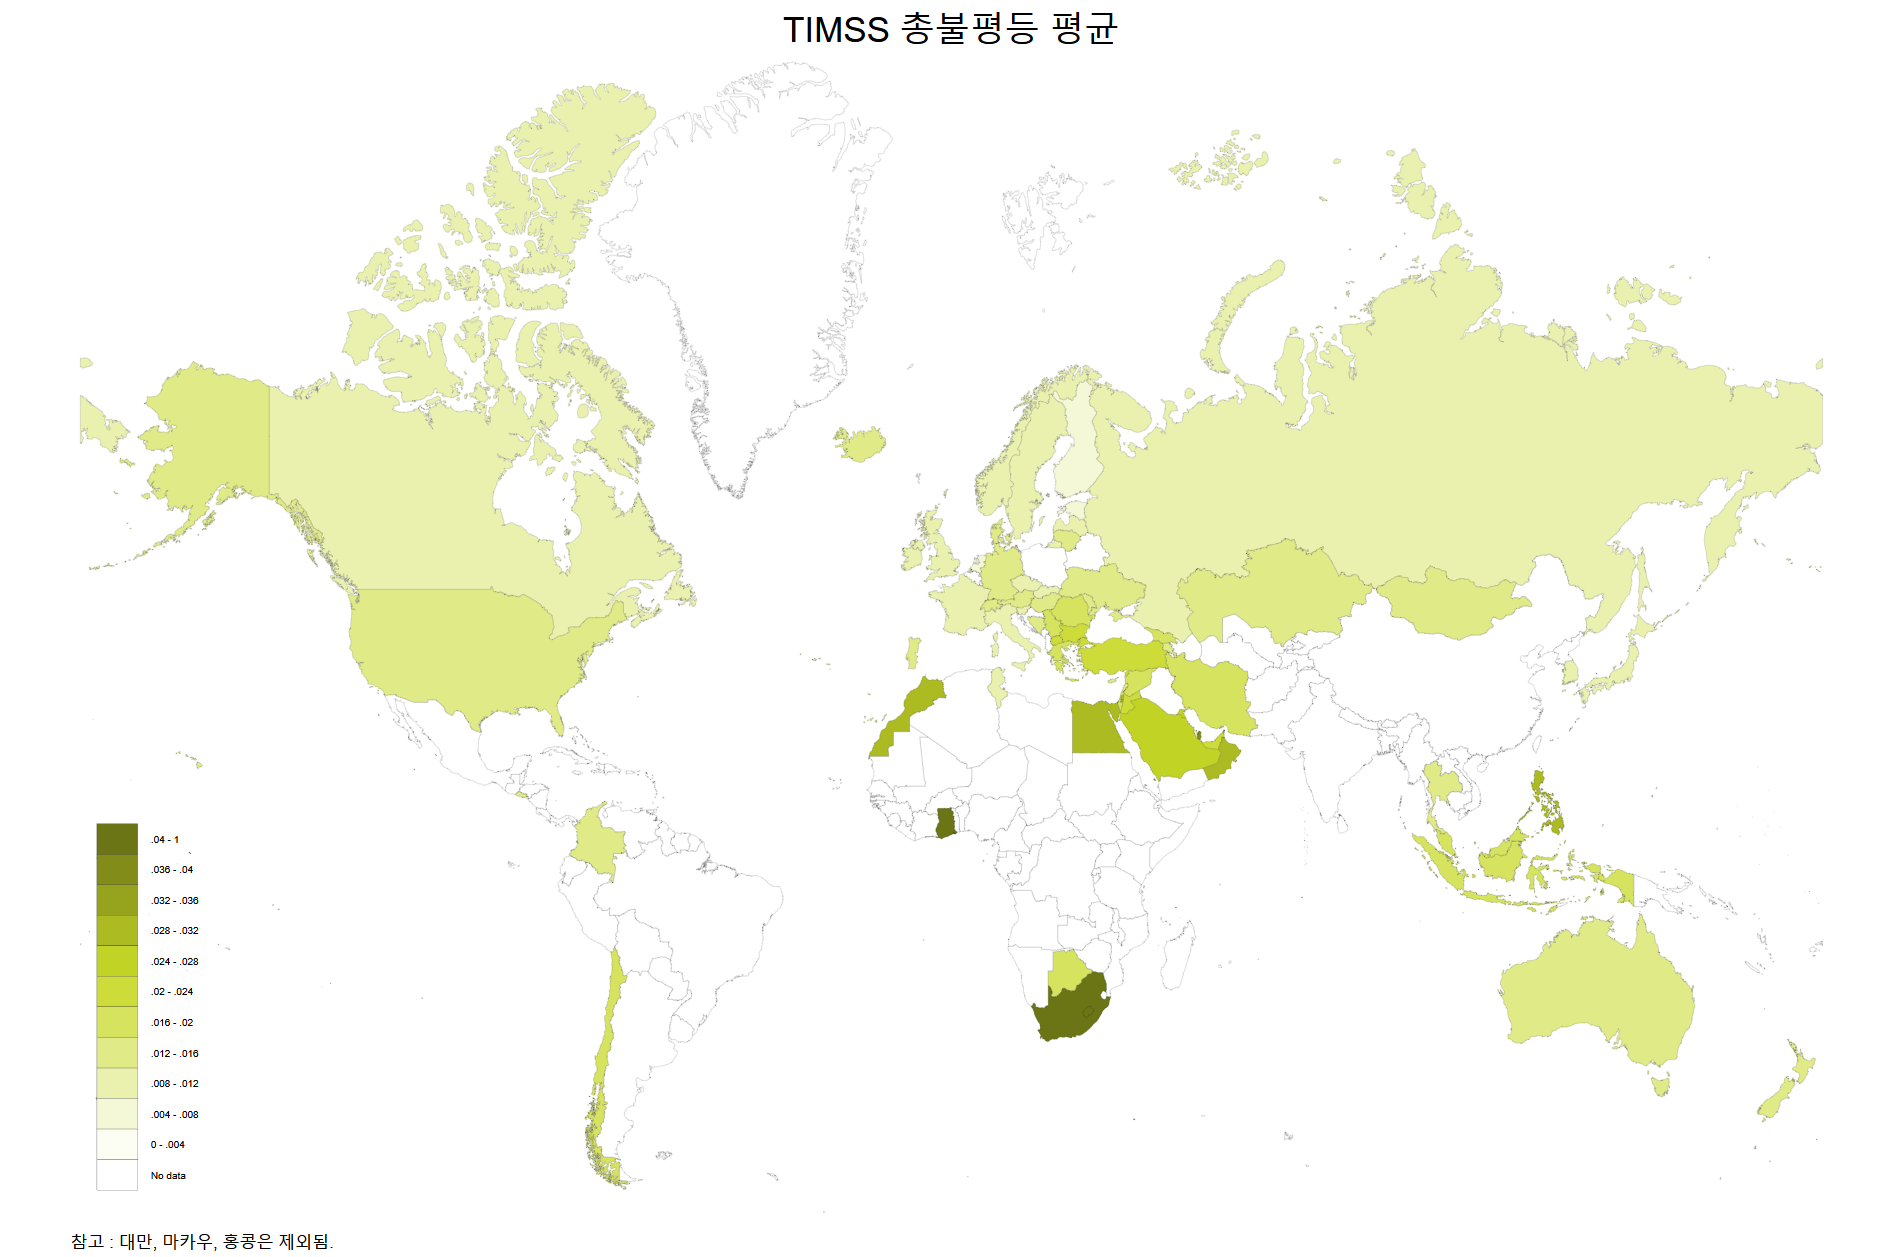
\includegraphics[width=\textwidth]{figure/map_bjttimss_mean.png}
    \label{fig:map_bjttimss_mean}
\end{figure}

\begin{figure}[htpb]
    \centering
    \caption{TIMSS 기회불평등의 비중}
    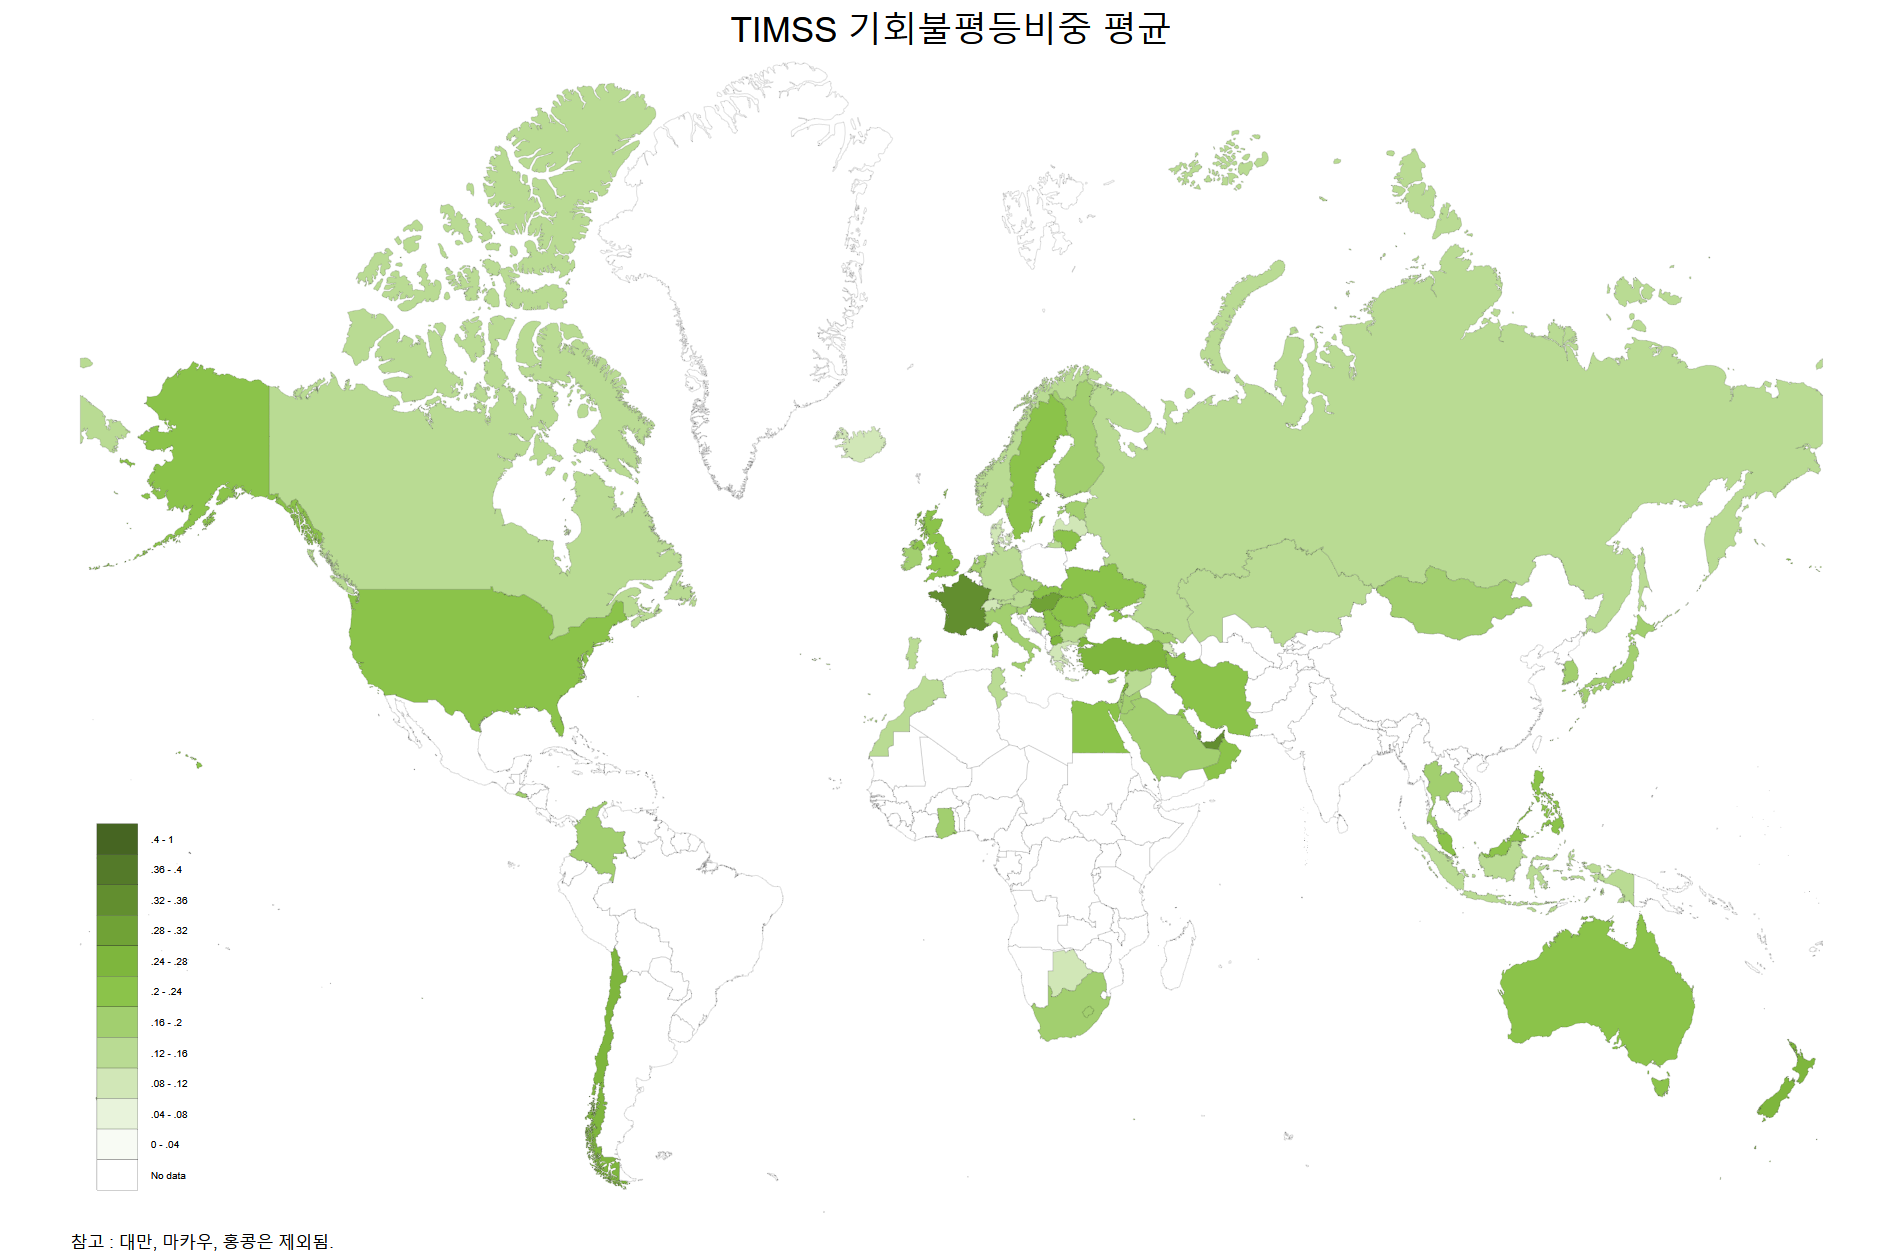
\includegraphics[width=\textwidth]{figure/map_bjrtimss_mean.png}
    \label{fig:map_bjrtimss_mean}
\end{figure}
    
\subsection{실증분석 모형}

본 연구에서 우리는 성장 회귀분석(growth regression)에서 일반적으로 사용하는 다음의 실증모형을 추정한다.
\begin{equation}
 \begin{aligned}
 \ln \left(Y_{i, t^{\prime}}\right)-\ln \left(Y_{i, t}\right)=& \delta_{1} I O P_{i, t}+\delta_{2} I O E_{i, t}+\beta_{1} \ln \left(Y_{i, t}\right)+X_{i, t} \beta_{2} \\
 &+\alpha_{i}+\tau_{t^{\prime}}+u_{i, t^{\prime}}
 \end{aligned}
 \label{eq:regbase}
\end{equation} 
 위 식에서 $i$는 국가를, $t$는 교육기회불평등의 측정연도이다. $t'$는 다음 조사시점을 의미하는데 개별 회귀분석마다 다를 수 있다. 연구의 편의를 위해 각 자료의 조사 주기를 따르기로 한다. 따라서 TIMSS의 경우 $t'=t+4$ 이고 PISA의 경우  $t'=t+3$이다. $Y_{i,t}$는 국가 $i$의 연도 $t$현재 1인당 GDP, $Y_{i,t'}$는 국가 $i$의 년도 $t'$현재 1인당 GDP를 표시한다. $\ln \left(Y_{i, t^{\prime}}\right)-\ln \left(Y_{i, t}\right)$ 는 국가 $i$의 연도 $t$에서 연도 $t'$까지 1인당 GDP의 성장률을 표시한다. 
 
우리는 먼저 식 (\ref{eq:regbase})의 종속변수로서 한 국가의 다음 조사기간의 경제성장률을 사용한다. 
$IOP_{i,t}$는 국가 $i$의 $t$연도 현재 교육 기회불평등 지수의 값이고, $IOE_{i,t}$ 는 총불평등에서 기회의 불평등에 의해 설명되지 않는 잔여불평등(노력 불평등의 대리 지표)을 표시한다. $X_{i,t}$는 국가 $i$의 $t$연도 현재 특성변수들로 인구의 로그값과 경제의 대외개방도를 가늠할 수 있는 투자재의 가격의 벡터이다. $\alpha _i$는 국가 고정효과, 그리고 $\tau _{t'}$는 연도 고정효과를 표시한다.

실제 회귀분석은 식 (\ref{eq:regbase})을 일부 수정한 식 (\ref{eq:regmod})에 대해 선형회귀분석(OLS), 패널 고정효과(fixed effect) 모형, 시스템 GMM(\citet{bnb98}) 방법을 적용함으로써 주요 계수들을 추정한다.

\begin{equation}
 \begin{aligned}
 \ln \left(Y_{i, t^{\prime}}\right)=& \delta_{1} I O P_{i, t}+\delta_{2} I O E_{i, t}+\left(\beta_{1}+1\right) \ln \left(Y_{i, t}\right)+X_{i, t} \beta_{2} \\
 &+\alpha_{i}+\tau_{t^{\prime}}+u_{i, t^{\prime}}
 \end{aligned}
 \label{eq:regmod}
\end{equation}

\section{분석 결과}
\subsection{그림을 통한 분석}

\begin{figure}
    \centering
    \caption{1인당GDP성장률과 교육의 총불평등; TIMSS}
    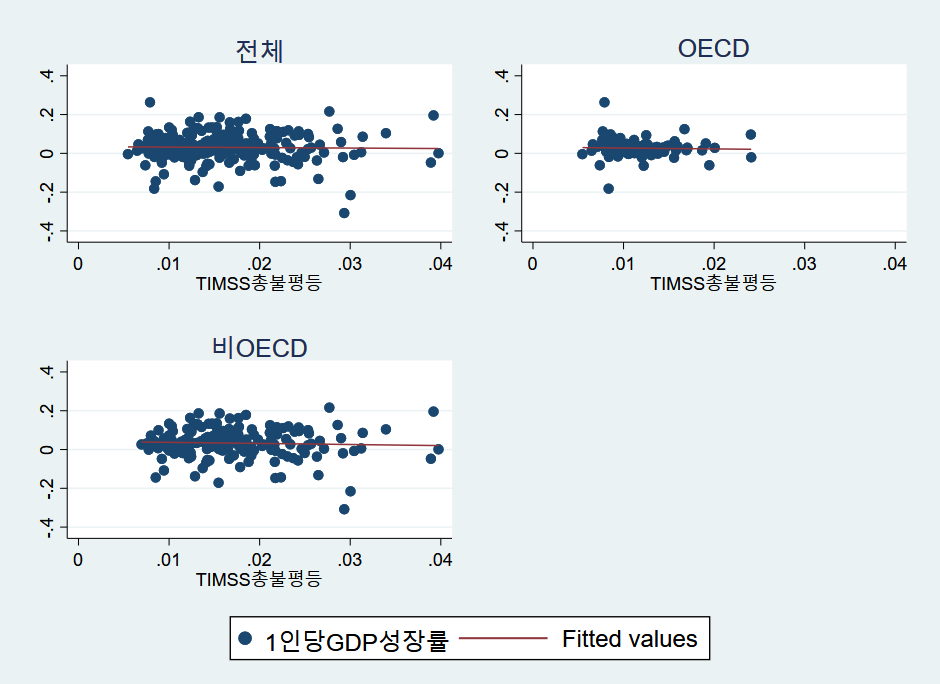
\includegraphics[width=\textwidth]{figure/scatter_pcgrowth_totmath_timss_noy.png}
    \label{fig:scatter_timss_pcgrowth_bjtmath_noy}
\end{figure}


\begin{figure}
    \centering
    \caption{1인당GDP성장률과 교육의 총불평등; PISA}
    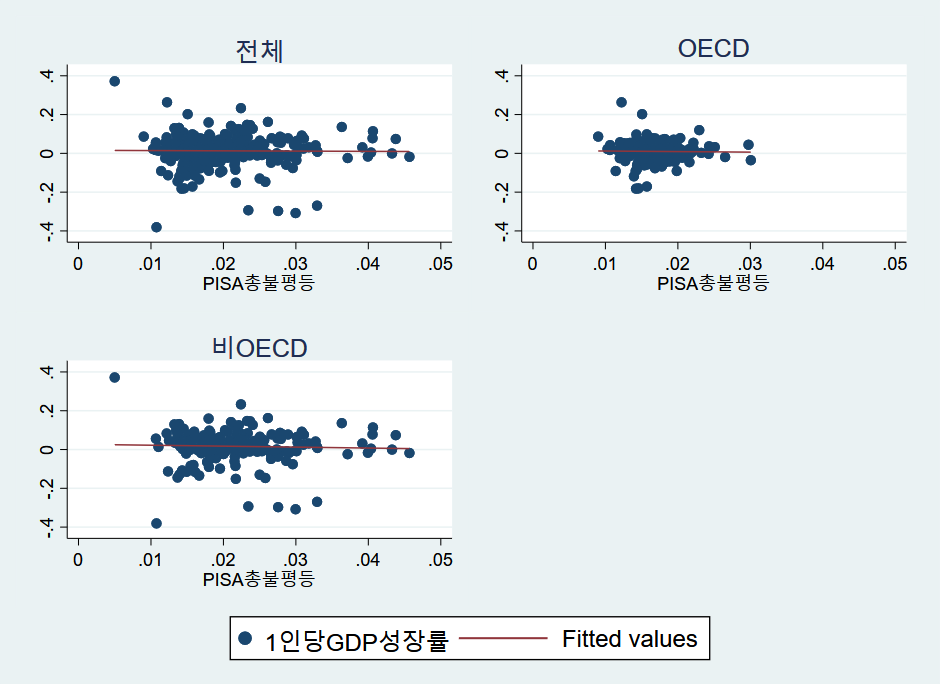
\includegraphics[width=\textwidth]{figure/scatter_pcgrowth_totmath_pisa_noy.png}
    \label{fig:scatter_pisa_pcgrowth_bjtmath_noy}
\end{figure}

그림 (\ref{fig:scatter_timss_pcgrowth_bjtmath_noy})과 (\ref{fig:scatter_pisa_pcgrowth_bjtmath_noy})의 Y축 변수로서 우리는 아래의 식 (\ref{eq:lfit})에 OLS를 적용해 구한 잔차(즉 $\ln \left(Y_{i, t'}\right)-\left[\widehat{\tau_{0}}+\widehat{\tau_{1}} \ln \left(Y_{i, t}\right)\right]$ )를 사용한다. 
한편 X축에 표시되어 있는 변수는 각국의 총불평등도 지수들이다.
\begin{equation}
\label{eq:lfit}
\ln \left(Y_{i, t'}\right)=\tau_{0}+\tau_{1} \ln \left(Y_{i, t}\right)+\epsilon_{i, t'}
\end{equation}
(\ref{fig:scatter_timss_pcgrowth_bjtmath_noy})에 (\ref{fig:scatter_pisa_pcgrowth_bjtmath_noy})에 의하면, 성적의 총불평등도는 대체로 경제성장에 부정적인 영향을 미치지만 그 효과는 다소 상이해 보인다.
이러한 부정적 영향은 OECD 국가들과 비OECD 국가들에서 동시에 관찰 된다.

\subsection{회귀 분석 결과}
본 절에서 우리는 본 연구의 자료를 사용해 불평등도와 경제성장 사이의 관계를 분석한 선행 실증연구들을 재현해 본다. 이를 통해 본 연구에서 사용하는 주요 자료들이 선행 연구에서 사용했던 자료와 비슷한 경향성을 보이는지를 확인할 수 있다.  표 (\ref{tab:pisa_reg1})에는 아래의 식 (\ref{eq:simplereg})를 추정한 결과가 제시되어 있다. 식 (\ref{eq:simplereg})는 불평등과 경제성장 사이의 관계를 다룬 많은 성장 회귀분석 연구에서 가장 빈번하게 사용되는 추정모형이다.
\begin{equation}
\label{eq:simplereg}
\ln \left(Y_{i, t'}\right)=\delta \operatorname{Ineq}_{i, t}+\left(\beta_{1}+1\right) \ln \left(Y_{i, t}\right)+X_{i, t} \beta_{2}+\alpha_{i}+\tau_{t'}+u_{i, t'}
\end{equation}
위 식에서 $Ineq_{i,t}$는 국가 $i$의 연도 $t$ 현재 성적의 총불평등도 지수이다. 식 (\ref{eq:simplereg})를 추정함으로써 우리는 TIMSS의 성적 불평등 지수를 사용하는 경우에도 전통적인 성장 회귀분석의 추정결과가 유사하게 나타나는지를 확인하고자 한다. 본 연구의 핵심 실증모형인 식 (\ref{eq:regmod})은 식 (\ref{eq:simplereg})의 $\delta Ineq_{i,t}$를 $\delta_{1} I O P_{i, t}+\delta_{2} I O E_{i, t}$와 같이 분해한 모형으로서 해석할 수 있다.
 
표 (\ref{tab:timss_reg1})의 (1)-(3)열은 전체 표본에 대해 각각 OLS, 패널 고정효과(Fixed Effects, FE), 시스템 GMM(Generalized Method of Moments) 추정법을 적용해 구한 추정치를 제시하고 있다.
OLS 추정법은 국가들 사이의 보이지 않는 이질성을 적절히 통제하지 못한다.
 이러한 국가 간 이질성의 문제를 통제하기 위해 패널 고정효과 모형을 사용하는 경우에도, $ln(Y_{i,t})$의 내생성 때문에 핵심 계수의 일치추정량을 구하기 어렵다고 알려져 있다.
위의 두 문제를 동시에 해결하기 위해 최근의 성장 회귀분석에서는 동태적 패널분석법(dynamic panel data analysis)의 하나인 시스템 GMM 추정법(\citet{bnb98})을 적용한다.
이하에서는 시스템 GMM 추정치들을 중심으로 분석결과를 설명하고자 한다.

%아울러 성적의 총불평등이 경제성장에 미치는 효과가 국가의 특성에 따라 서로 상이한지를 검증하기 위해 우리는 식 (\ref{eq:regmod})의 불평등부분을 $\delta$ Ineq $_{i, t}=\delta_{N} N O E C D_{i} \times$ Ineq $_{i, t}+\delta_{O} O E C D_{i} \times$ Ineq $_{i, t}$ 와 같이 분해한다.
%여기에서 $OECD_i$ 는 국가 $i$가 $t$년도 현재 OECD 가입국이면 1, 그렇지 않으면 0을 취하는 더미변수이고, $NOECD_i$는 반대로 비OECD 국가에 대한 더미변수 이다.
%표 (\ref{tab:timss_reg1})의 (4)-(6)열에는 전체 표본을 비 OECD 국가 집단과 OECD 국가 집단으로 구분한 경우의 추정치가 제시되어 있다.  

\label{ans6}
아울러 교육의 총불평등이 경제성장에 미치는 효과가 국가의 특성에 따라 서로 상이한지를 검증하기 위해 우리는 식 (\ref{eq:simplereg})에 OECD 가입여부에 대한 가변수를 이용한 변형을 한다.
불평등지수의 항인 $\delta$ Ineq $_{i, t}$를 $\delta_{1} Ineq _{i, t}  + \delta _{2} O E C D_{i} \times$ Ineq $_{i, t} + \delta_{3} O E C D_{i} $로 대체한다.
여기에서 $OECD_i$ 는 국가 $i$가 $t$년도 현재 OECD 가입국이면 1, 그렇지 않으면 0을 취하는 가변수이다.
따라서 $\delta _ 1$은 개별 국가의 특성에 상관없이 불평등이 경제성장에 미치는 영향을 나타낸다. 
$\delta _ 2$는 비교적 발전이 진행된 OECD 가입국에서 불평등정도가 경제성장에 미치는 영향을 각각 나타낸다.
$\delta _ 3$는 OECD로 가입여부로 나타낸 국가의 발전정도가 경제성장에 미치는 영향을 나타낸다.
표 (\ref{tab:timss_reg1})의 (4)-(6)열에는 전체 표본을 비 OECD 국가 집단과 OECD 국가 집단으로 구분한 경우의 추정치가 제시되어 있다.  

\begin{table}[htbp]\centering
\def\sym#1{\ifmmode^{#1}\else\(^{#1}\)\fi}
\caption{회귀분석 결과 : TIMSS, 총불평등 \label{tab:timss_reg1}}
\resizebox{\textwidth}{!}{
\begin{tabular}{l*{6}{c}}
\hline\hline
                    &\multicolumn{1}{c}{(1)}&\multicolumn{1}{c}{(2)}&\multicolumn{1}{c}{(3)}&\multicolumn{1}{c}{(4)}&\multicolumn{1}{c}{(5)}&\multicolumn{1}{c}{(6)}\\
                    &\multicolumn{1}{c}{OLS}&\multicolumn{1}{c}{FE}&\multicolumn{1}{c}{Sys. GMM}&\multicolumn{1}{c}{OLS}&\multicolumn{1}{c}{FE}&\multicolumn{1}{c}{Sys. GMM}\\
\hline
총불평등          &      -1.172\sym{*}  &       0.199         &      -4.649\sym{*}  &      -1.220\sym{*}  &      0.0398         &      -3.828\sym{*}  \\
                    &     (0.666)         &     (0.803)         &     (2.427)         &     (0.707)         &     (0.802)         &     (2.256)         \\
[1em]
OECD $\times$ 총불평등&                     &                     &                     &       6.624         &       13.40\sym{**} &       13.31\sym{*}  \\
                    &                     &                     &                     &     (4.072)         &     (6.678)         &     (7.506)         \\
[1em]
OECD              &                     &                     &                     &     -0.0595         &      -0.151         &    -0.00967         \\
                    &                     &                     &                     &    (0.0526)         &    (0.0997)         &     (0.118)         \\
[1em]
ln1인당GDP        &       0.927\sym{***}&       0.570\sym{***}&       0.807\sym{***}&       0.925\sym{***}&       0.570\sym{***}&       0.775\sym{***}\\
                    &    (0.0146)         &    (0.0550)         &    (0.0652)         &    (0.0148)         &    (0.0549)         &    (0.0731)         \\
[1em]
투자재가격        &      0.0640         &      -0.148         &      0.0628         &      0.0599         &      -0.138         &    -0.00241         \\
                    &    (0.0491)         &    (0.0901)         &     (0.105)         &    (0.0551)         &    (0.0898)         &    (0.0921)         \\
[1em]
ln인구            &    -0.00920         &      -0.320\sym{***}&      -0.174\sym{**} &     -0.0112\sym{*}  &      -0.327\sym{***}&      -0.222\sym{***}\\
                    &   (0.00606)         &    (0.0988)         &    (0.0714)         &   (0.00670)         &    (0.0985)         &    (0.0811)         \\
[1em]
Constant            &       0.842\sym{***}&       5.384\sym{***}&       2.518\sym{***}&       0.864\sym{***}&       5.402\sym{***}&       2.918\sym{***}\\
                    &     (0.135)         &     (0.641)         &     (0.670)         &     (0.139)         &     (0.644)         &     (0.726)         \\
\hline
r2                  &       0.974         &       0.820         &                     &       0.975         &       0.824         &                     \\
관측수                   &         238         &         238         &         238         &         238         &         238         &         238         \\
국가수                 &                     &          71         &          71         &                     &          71         &          71         \\
\hline\hline
\multicolumn{7}{l}{\footnotesize 괄호안은 표준오차.}\\
\multicolumn{7}{l}{\footnotesize \sym{*} \(p<0.10\), \sym{**} \(p<0.05\), \sym{***} \(p<0.01\)}\\
\end{tabular}}
\end{table}


먼저 TIMSS의 경우를 살펴본다.
회귀분석에는 총 71개국에서 238개 불평등 지수가 측정되어 한 국가당 약 3회 정도의 관측치가 사용되었다.
ln1인당GDP의 계수는 식 (\ref{eq:simplereg})에 의하면 1이 더해진 값임에 주의해야 한다. 따라서 표에 제시된 계수들에서 1을 차감한 값이 추정된 값으로 1인당 GDP가 이미 높은 수준일수록 경제성장률이 낮다는 상식에 부합한다.
표 (\ref{tab:timss_reg1})의 (3)열을 보면, 학업성취도의 총불평등도는 4년 후의 1인당 GDP에 유의미한 부정적 관계(추정치 -4.649)를 가진다.
OECD 가입여부를 구분해서 살펴보는 (6)열에 의하면, 학업성취도의 불평등은 -3.828로 유의미한 음의 관계를 보이는 반면 OECD국가들에서는 13.31로 유의미한 양의 상관관계를 나타냈다. 
OECD 국가라는 사실은 유의미한 영향을 주지 못하는 것으로 보였다.
이는 국가별 발전정도에 따라 불평등이 경제성장에 미치는 영향이 정 반대로 나타날 수 있음을 보여주고 있다.
이 추정치를 한국의 경우를 예로 들어 해석하면 다음과 같다.
2003년 한국의 총불평등은 0.0071인데 2007년은 0.0095로 0.0024 증가 하였다.
 증가분에 추정된 계수값 13.31을 곱한 수치는 약 0.032로 수학 학업성취도의 총불평등 증가는 한국의 4년간 경제성장률을 약 3.2\%포인트 상승시켰을 것으로 추정된다.
 실제 한국의 2007년에서 2011년 사이 경제성장률은 약 2.3\% 이었으므로, 2007년도의 한국의 학업성취도 불평등도가 2003년 수준으로 유지되었다면, 2007년과 2011년 사이의 경제성장률은 -0.9\%이었을 것으로 추정된다.

\begin{table}[htbp]\centering
\def\sym#1{\ifmmode^{#1}\else\(^{#1}\)\fi}
\caption{회귀분석 결과 : TIMSS, 기회 vs. 잔여불평등 \label{tab:timss_reg2}}
\resizebox{\textwidth}{!}{
\begin{tabular}{l*{6}{c}}
\hline\hline
                    &\multicolumn{1}{c}{(1)}&\multicolumn{1}{c}{(2)}&\multicolumn{1}{c}{(3)}&\multicolumn{1}{c}{(4)}&\multicolumn{1}{c}{(5)}&\multicolumn{1}{c}{(6)}\\
                    &\multicolumn{1}{c}{OLS}&\multicolumn{1}{c}{FE}&\multicolumn{1}{c}{Sys. GMM}&\multicolumn{1}{c}{OLS}&\multicolumn{1}{c}{FE}&\multicolumn{1}{c}{Sys. GMM}\\
\hline
기회불평등        &      -1.750         &      -1.374         &      -16.65\sym{**} &      -1.553         &      -2.401         &      -15.11\sym{*}  \\
                    &     (5.203)         &     (5.169)         &     (7.331)         &     (5.534)         &     (5.291)         &     (7.734)         \\
[1em]
잔여불평등        &      -1.053         &       0.483         &      -2.334         &      -1.184         &       0.475         &      -1.620         \\
                    &     (1.204)         &     (1.222)         &     (2.566)         &     (1.292)         &     (1.231)         &     (2.339)         \\
[1em]
OECD $\times$ 기회불평등&                     &                     &                     &      -6.446         &       13.03         &      -2.922         \\
                    &                     &                     &                     &     (12.79)         &     (20.68)         &     (19.52)         \\
[1em]
OECD $\times$ 잔여불평등&                     &                     &                     &       10.34         &       13.88\sym{*}  &       19.41\sym{**} \\
                    &                     &                     &                     &     (6.320)         &     (8.089)         &     (7.735)         \\
[1em]
OECD              &                     &                     &                     &     -0.0637         &      -0.156         &     -0.0299         \\
                    &                     &                     &                     &    (0.0553)         &     (0.101)         &     (0.114)         \\
[1em]
ln1인당GDP        &       0.928\sym{***}&       0.568\sym{***}&       0.817\sym{***}&       0.925\sym{***}&       0.567\sym{***}&       0.780\sym{***}\\
                    &    (0.0145)         &    (0.0553)         &    (0.0671)         &    (0.0149)         &    (0.0554)         &    (0.0764)         \\
[1em]
투자재가격        &      0.0630         &      -0.149         &      0.0520         &      0.0587         &      -0.138         &     0.00736         \\
                    &    (0.0480)         &    (0.0904)         &    (0.0948)         &    (0.0540)         &    (0.0915)         &    (0.0841)         \\
[1em]
ln인구            &    -0.00923         &      -0.318\sym{***}&      -0.178\sym{**} &     -0.0111\sym{*}  &      -0.325\sym{***}&      -0.224\sym{***}\\
                    &   (0.00608)         &    (0.0993)         &    (0.0731)         &   (0.00668)         &    (0.0993)         &    (0.0824)         \\
[1em]
Constant            &       0.839\sym{***}&       5.393\sym{***}&       2.446\sym{***}&       0.869\sym{***}&       5.419\sym{***}&       2.869\sym{***}\\
                    &     (0.134)         &     (0.644)         &     (0.684)         &     (0.140)         &     (0.648)         &     (0.750)         \\
\hline
r2                  &       0.974         &       0.820         &                     &       0.975         &       0.825         &                     \\
관측수                   &         238         &         238         &         238         &         238         &         238         &         238         \\
국가수                 &                     &          71         &          71         &                     &          71         &          71         \\
\hline\hline
\multicolumn{7}{l}{\footnotesize 괄호안은 표준오차.}\\
\multicolumn{7}{l}{\footnotesize \sym{*} \(p<0.10\), \sym{**} \(p<0.05\), \sym{***} \(p<0.01\)}\\
\end{tabular}}
\end{table}

표 \ref{tab:timss_reg2}는 표 \ref{tab:timss_reg1}의 총불평등을 기회불평등과 잔여불평등으로 분해하여 회귀분석한 결과이다.
(3)열을 보면, 학업성취도의 기회불평등도의 계수는 -16.65로 4년 후의 1인당 GDP에 유의미한 부정적 관계를 가진다.
OECD 가입여부를 구분해서 살펴보는 (6)열에 의하면, 기회불평등의 계수값은 -15.11로 기회불평등이 커질수록 경제성장에 부정적 영향을 주는 것을 확인했다.
OECD 국가들의 경우로 제한해서 살펴보면 학업성취도의 기회불평등은 OECD국가들에서 유의미한 영향을 주지 못하였다. 
반면 잔여불평등은 계수값이 19.41으로 유의미한 긍정적 영향을 주는 것을 확인하였다.
다시 말해, 앞서 학업성취도의 불평등이 커질수록 경제성장에 긍정적 영향을 준다는 결과는 환경에서 비롯되지 않은 개인의 순수한 노력을 포함한 요소에 의한 성적 격차의 증가가 경제성장에 긍정적 영향을 준다는 의미이다.

\centering
\def\sym#1{\ifmmode^{#1}\else\(^{#1}\)\fi}
\caption{PISA 총불평등\label{tab:pisasimp}}
\begin{tabular}{l*{6}{c}}
\toprule
                    &\multicolumn{1}{c}{(1)}&\multicolumn{1}{c}{(2)}&\multicolumn{1}{c}{(3)}&\multicolumn{1}{c}{(4)}&\multicolumn{1}{c}{(5)}&\multicolumn{1}{c}{(6)}\\ &\multicolumn{1}{c}{OLS}&\multicolumn{1}{c}{FE}&\multicolumn{1}{c}{Sys. GMM}&\multicolumn{1}{c}{OLS}&\multicolumn{1}{c}{FE}&\multicolumn{1}{c}{Sys. GMM}\\
\midrule
총불평등          &      -3.248\sym{***}&      -4.625\sym{***}&      -2.332         &                     &                     &                     \\
                    &     [-2.99]         &     [-3.27]         &     [-0.58]         &                     &                     &                     \\
\addlinespace
OECD$ \times$ 총불평등&                     &                     &                     &      -3.562\sym{***}&      -2.107         &       0.737         \\
                    &                     &                     &                     &     [-2.70]         &     [-0.95]         &      [0.12]         \\
\addlinespace
비OECD$ \times$ 총불평등&                     &                     &                     &      -3.268\sym{***}&      -4.875\sym{***}&      -3.968         \\
                    &                     &                     &                     &     [-3.00]         &     [-3.43]         &     [-1.08]         \\
\midrule
r2                  &       0.980         &       0.803         &                     &       0.980         &       0.804         &                     \\
N                   &         334         &         334         &         334         &         334         &         334         &         334         \\
N\_g                 &                     &          77         &          77         &                     &          77         &          77         \\
\bottomrule
\multicolumn{7}{l}{\footnotesize \textit{t} statistics in brackets}\\
\multicolumn{7}{l}{\footnotesize \sym{*} \(p<0.10\), \sym{**} \(p<0.05\), \sym{***} \(p<0.01\)}\\
\end{tabular}


지금부터는 PISA 자료를 이용하여 문해력의 불평등이 경제성장에 미치는 영향을 살펴본다.
PISA 자료에는 77개 국에서 총 358회의 불평등지수를 측정하였으며 이는 국가별로 평균 4회에 해당한다.
PISA로 측정한 문해력의 불평등과 경제성장간의 관계는 앞서 살펴본 학업성취도의 불평등과는 다른 모습을 보인다.
표 (\ref{tab:pisa_reg1})에 제시된 분석 결과를 요약하면 다음과 같다.
OLS와 FE 추정방법을 사용하는 경우에도 유의미했던 부정적 관계가 시스템 GMM 추정법을 사용할 경우 유의성이 없는 것으로 나타났다.
이는 TIMSS의 경우 유의미한 부정적 관계를 보인것과 상이하다.
(6)열에 의하면, 문해력의 불평등은 (3)열의 경우와 마찬가지로 OECD 가입 여부를 나누어 고려하더라도 유의미한 영향을 주지 못하는 것으로 나타났다.

\begin{table}[htbp]\centering
\def\sym#1{\ifmmode^{#1}\else\(^{#1}\)\fi}
\caption{회귀분석 결과 : PISA, 기회 vs. 잔여불평등 \label{tab:pisa_reg2}}
\resizebox{\textwidth}{!}{
\begin{tabular}{l*{6}{c}}
\hline\hline
                    &\multicolumn{1}{c}{(1)}&\multicolumn{1}{c}{(2)}&\multicolumn{1}{c}{(3)}&\multicolumn{1}{c}{(4)}&\multicolumn{1}{c}{(5)}&\multicolumn{1}{c}{(6)}\\
                    &\multicolumn{1}{c}{OLS}&\multicolumn{1}{c}{FE}&\multicolumn{1}{c}{Sys. GMM}&\multicolumn{1}{c}{OLS}&\multicolumn{1}{c}{FE}&\multicolumn{1}{c}{Sys. GMM}\\
\hline
기회불평등        &      -2.924         &      -0.375         &       9.860         &      -6.456         &       1.176         &       4.884         \\
                    &     (4.964)         &     (6.002)         &     (11.29)         &     (7.345)         &     (7.213)         &     (12.28)         \\
[1em]
잔여불평등        &      -3.371\sym{**} &      -5.716\sym{***}&      -6.400\sym{*}  &      -2.601         &      -6.889\sym{***}&      -6.563         \\
                    &     (1.680)         &     (2.060)         &     (3.871)         &     (2.184)         &     (2.271)         &     (4.344)         \\
[1em]
OECD $\times$ 기회불평등&                     &                     &                     &       9.16         &      -6.279         &       7.417         \\
                    &                     &                     &                     &     (8.644)         &     (12.67)         &     (15.50)         \\
[1em]
OECD $\times$ 잔여불평등&                     &                     &                     &      -1.457         &       9.365         &       1.302         \\
                    &                     &                     &                     &     (3.482)         &     (5.883)         &     (7.058)         \\
[1em]
OECD              &                     &                     &                     &     -0.0348         &     -0.0713         &      0.0326         \\
                    &                     &                     &                     &    (0.0456)         &    (0.0791)         &     (0.158)         \\
[1em]
ln1인당GDP        &       0.931\sym{***}&       0.599\sym{***}&       0.812\sym{***}&       0.936\sym{***}&       0.597\sym{***}&       0.790\sym{***}\\
                    &    (0.0165)         &    (0.0423)         &    (0.0655)         &    (0.0180)         &    (0.0424)         &    (0.0754)         \\
[1em]
투자재가격        &     -0.0549         &      -0.140\sym{**} &      0.0155         &     -0.0381         &      -0.154\sym{**} &     -0.0368         \\
                    &    (0.0468)         &    (0.0603)         &     (0.162)         &    (0.0442)         &    (0.0610)         &     (0.110)         \\
[1em]
ln인구            &    -0.00779\sym{**} &      -0.200\sym{**} &      -0.192\sym{**} &    -0.00680\sym{**} &      -0.221\sym{**} &      -0.195\sym{**} \\
                    &   (0.00322)         &    (0.0899)         &    (0.0904)         &   (0.00329)         &    (0.0906)         &    (0.0881)         \\
[1em]
Constant            &       0.972\sym{***}&       4.901\sym{***}&       2.584\sym{***}&       0.922\sym{***}&       4.977\sym{***}&       2.815\sym{***}\\
                    &     (0.155)         &     (0.530)         &     (0.709)         &     (0.168)         &     (0.535)         &     (0.753)         \\
\hline
r2                  &       0.980         &       0.803         &                     &       0.980         &       0.806         &                     \\
관측수                   &         334         &         334         &         334         &         334         &         334         &         334         \\
국가수                 &                     &          77         &          77         &                     &          77         &          77         \\
\hline\hline
\multicolumn{7}{l}{\footnotesize  괄호안은 표준오차.}\\
\multicolumn{7}{l}{\footnotesize \sym{*} \(p<0.10\), \sym{**} \(p<0.05\), \sym{***} \(p<0.01\)}\\
\end{tabular}}
\end{table}

표 (\ref{tab:pisa_reg2})는 앞서와 마찬가지로 표 (\ref{tab:pisa_reg1})의 결과에서 총불평등을 기회불평등과 잔여불평등으로 나누어 분석한 결과이다.
(3)열에 제시되어 있는 추정치에 의하면, 문해력의 기회불평등도는 3년 후의 1인당 GDP에 유의하지 않지만 긍정적인 영향을 준다.
반면 잔여불평등은 계수값 -6.400으로 유의미하게 부정적인 영향을 준다.
하지만 (6)열에 의하면, OECD 가변수와 두 불평등지수와 OECD 가변수와의 교차항을 고려하여 추정을 한다면 문해력의 불평등이 경제성장에 주는 유의미한 영향을 없는 것을 알 수 있다.

\section{강건성 검증}

이번 절에서는 앞서 제시한 회귀분석 결과에 대한 강건성을 두 가지 측면에서 검증한다. 이 절의 모든 회귀분석 결과는 시스템 GMM 추정법을 이용한 결과만을 제시한다.
먼저 \citet{mnr13}과 \citet{kno17}에서와 같이 \citet{fng11}의 관측되지 않은 환경으로 인한 성취를 고려하지 않은 기회불평등 지수(이하 FG지수)를 이용한 회귀분석 결과를 제시하여 본 연구의 결과와 비교한다.
그래서 \citet{betl12}의 방법을 이용할 경우(이하 BJ지수)와 비교하여 환경의 영향을 더욱 적극적으로 고려하는 기회불평등 추정 방법이 분석 결과에 어떤 영향을 주는지 알아본다.

다음으로 종속변수인 성장률을 측정하는 시기를 3년, 4년, 5년으로 각각 다르게 한 경우의 회귀분석 결과를 동시에 비교한다.
본 연구의 대상자료인 TIMSS와 PISA가 각각 4년과 3년이라는 상이한 조사주기를 가지는 점이 연구결과에 어떤 영향을 주는지 검증한다.

표 (\ref{tab:timss_reg_rob1})은 TIMSS 자료를 대상으로 동일한 회귀분석에 대하여 불평등 지수를 BJ지수와 FG지수를 각각 대입했을때의 결과를 보여주고 있다.
총불평등을 대상으로 하는 (1)열과 (2)열이나, OECD 국가를 구분해서 총불평등이 경제성장에 주는 영향을 분석한 (3)열과 (4)열의 경우처럼 몇몇 사례에서 분석결과의 유의성 여부가 바뀌는 경우가 존재한다.
하지만 전체적으로 BJ지수의 주요 결과가 FG지수로 분석했을때의 결과와 모순되지 않음을 알 수 있다.  

\begin{table}[htbp]\centering
\def\sym#1{\ifmmode^{#1}\else\(^{#1}\)\fi}
\caption{회귀분석 결과 : TIMSS, 지수비교 \label{tab:timss_reg_rob1}}
\resizebox{\textwidth}{!}{
\begin{tabular}{l*{8}{c}}
\hline\hline
                    &\multicolumn{1}{c}{(1)}&\multicolumn{1}{c}{(2)}&\multicolumn{1}{c}{(3)}&\multicolumn{1}{c}{(4)}&\multicolumn{1}{c}{(5)}&\multicolumn{1}{c}{(6)}&\multicolumn{1}{c}{(7)}&\multicolumn{1}{c}{(8)}\\
                    &\multicolumn{1}{c}{BJ지수}&\multicolumn{1}{c}{FG지수}&\multicolumn{1}{c}{BJ지수}&\multicolumn{1}{c}{FG지수}&\multicolumn{1}{c}{BJ지수}&\multicolumn{1}{c}{FG지수}&\multicolumn{1}{c}{BJ지수}&\multicolumn{1}{c}{FG지수}\\
\hline
총불평등          &      -4.649\sym{*}  &       -0.792          &      -3.828\sym{*}  &   -0.690           &                     &                     &                     &                     \\
                    &     (2.427)         &      (0.938)         &     (2.256)         &     (0.877)        &                     &                     &                     &                     \\
[1em]
OECD $\times$ 총불평등&                     &                     &       13.31\sym{*}  &        20.44\sym{***}&                  &                     &                     &                     \\
                    &                     &                     &     (7.506)         &      (7.028)          &                     &                     &                     &                     \\
[1em]
기회불평등        &                     &                     &                     &                     &      -16.65\sym{**} &       -14.68        &      -15.11\sym{*}  &    -16.62\sym{*}      \\
                    &                     &                     &                     &                     &     (7.331)         &      (10.62)        &     (7.734)         &   (9.189)            \\
[1em]
잔여불평등        &                     &                     &                     &                     &      -2.334         &      0.316         &      -1.620         &    0.602          \\
                    &                     &                     &                     &                     &     (2.566)         &    (1.295)         &     (2.339)         &  (0.995)        \\
[1em]
OECD $\times$ 기회불평등&                     &                     &                     &                     &                     &                     &      -2.922         & -17.66                            \\
                    &                     &                     &                     &                     &                     &                     &     (19.52)         &     (26.57)                       \\
[1em]                                                                                                                                                                                             
OECD $\times$ 잔여불평등&                     &                     &                     &                     &                     &                     &       19.41\sym{**} & 30.08\sym{***}                    \\
                    &                     &                     &                     &                     &                     &                     &     (7.735)         &     (8.551)                       \\
[1em]
OECD              &                     &                     &    -0.00967         &     -0.0881         &                     &                     &     -0.0299         &     -0.0852         \\
                    &                     &                     &     (0.118)         &     (0.122)         &                     &                     &     (0.114)         &     (0.125)         \\
[1em]
ln1인당GDP        &       0.807\sym{***}&       0.819\sym{***}&       0.775\sym{***}&       0.787\sym{***}&       0.817\sym{***}&       0.826\sym{***}&       0.780\sym{***}&       0.782\sym{***}\\
                    &    (0.0652)         &    (0.0606)         &    (0.0731)         &    (0.0689)         &    (0.0671)         &    (0.0597)         &    (0.0764)         &    (0.0699)         \\
[1em]
투자재가격        &      0.0628         &       0.111         &    -0.00241         &      0.0208         &      0.0520         &       0.114         &     0.00736         &      0.0388         \\
                    &     (0.105)         &     (0.107)         &    (0.0921)         &    (0.0906)         &    (0.0948)         &     (0.101)         &    (0.0841)         &    (0.0856)         \\
[1em]
ln인구            &      -0.174\sym{**} &      -0.160\sym{**} &      -0.222\sym{***}&      -0.214\sym{***}&      -0.178\sym{**} &      -0.157\sym{**} &      -0.224\sym{***}&      -0.214\sym{***}\\
                    &    (0.0714)         &    (0.0687)         &    (0.0811)         &    (0.0807)         &    (0.0731)         &    (0.0688)         &    (0.0824)         &    (0.0820)         \\
[1em]
Constant            &       2.518\sym{***}&       2.281\sym{***}&       2.918\sym{***}&       2.699\sym{***}&       2.446\sym{***}&       2.215\sym{***}&       2.869\sym{***}&       2.745\sym{***}\\
                    &     (0.670)         &     (0.628)         &     (0.726)         &     (0.690)         &     (0.684)         &     (0.622)         &     (0.750)         &     (0.700)         \\
\hline
r2                  &                     &                     &                     &                     &                     &                     &                     &                     \\
관측수                   &         238         &         238         &         238         &         238         &         238         &         238         &         238         &         238         \\
국가수                 &          71         &          71         &          71         &          71         &          71         &          71         &          71         &          71         \\
\hline\hline
\multicolumn{9}{l}{\footnotesize  괄호안은 표준오차.}\\
\multicolumn{9}{l}{\footnotesize \sym{*} \(p<0.10\), \sym{**} \(p<0.05\), \sym{***} \(p<0.01\)}\\
\end{tabular}}
\end{table}


표 (\ref{tab:timss_reg_rob2})은 TIMSS 자료를 대상으로 동일한 회귀분석에 대하여 불평등 지수를 BJ지수와 FG지수를 각각 대입했을때의 결과를 보여주고 있다.
PISA 자료로 동일하게 지수간 비교를 시행한 표 (\ref{tab:pisa_reg_rob1})의 결과 역시 \citet{betl12}의 방법을 적용한 불평등지수 계산이 결과에 영향을 주지 않음을 보여주고 있다.

\begin{table}[htbp]\centering
\def\sym#1{\ifmmode^{#1}\else\(^{#1}\)\fi}
\caption{회귀분석 결과 : PISA, 지수비교 \label{tab:pisa_reg_rob1}}
\resizebox{\textwidth}{!}{
\begin{tabular}{l*{8}{c}}
\hline\hline
                    &\multicolumn{1}{c}{(1)}&\multicolumn{1}{c}{(2)}&\multicolumn{1}{c}{(3)}&\multicolumn{1}{c}{(4)}&\multicolumn{1}{c}{(5)}&\multicolumn{1}{c}{(6)}&\multicolumn{1}{c}{(7)}&\multicolumn{1}{c}{(8)}\\
                    &\multicolumn{1}{c}{BJ지수}&\multicolumn{1}{c}{FG지수}&\multicolumn{1}{c}{BJ지수}&\multicolumn{1}{c}{FG지수}&\multicolumn{1}{c}{BJ지수}&\multicolumn{1}{c}{FG지수}&\multicolumn{1}{c}{BJ지수}&\multicolumn{1}{c}{FG지수}\\
\hline
총불평등          &      -2.332         &       -1.913    &      -3.770    &      -3.056   &                     &                     &                     &                     \\
                    &     (4.008)         &      (3.834)    &     (4.151)    &     (3.885)   &                     &                     &                     &                     \\
[1em]
OECD $\times$ 총불평등&                     &                     &       3.211         &        1.839   &                     &                     &                     &                     \\
                    &                     &                     &     (4.288)         &      (4.246)   &                     &                     &                     &                     \\
[1em]
기회불평등        &                     &                     &                     &                     &       9.860         &        20.70         &       4.884         &     13.91                        \\
                    &                     &                     &                     &                     &     (11.29)         &      (14.49)         &     (12.28)         &   (13.06)                        \\
[1em]                                                                                                                                                                                          
잔여불평등        &                     &                     &                     &                     &      -6.400\sym{*}  &       -7.144\sym{*}  &      -6.563         &    -6.774\sym{*}                 \\
                    &                     &                     &                     &                     &     (3.871)         &      (3.673)         &     (4.344)         &   (3.861)                        \\
[1em]
OECD $\times$ 기회불평등&        &        &       &                     &                     &                     &       7.417         &        10.52                     \\
                    &        &        &       &                     &                     &                     &     (15.50)         &      (15.15)                     \\
[1em]                                                                                                                                                     
OECD $\times$ 잔여불평등&        &        &       &                     &                     &                     &       1.302         &       -1.214                     \\
                    &        &        &       &                     &                     &                     &     (7.058)         &      (5.660)                     \\
[1em]
OECD              &                     &                     &      0.0297         &      0.0523         &                     &                     &      0.0326         &      0.0499         \\
                    &                     &                     &     (0.154)         &     (0.149)         &                     &                     &     (0.158)         &     (0.158)         \\
[1em]
ln1인당GDP        &       0.817\sym{***}&       0.819\sym{***}&       0.793\sym{***}&       0.793\sym{***}&       0.812\sym{***}&       0.806\sym{***}&       0.790\sym{***}&       0.789\sym{***}\\
                    &    (0.0633)         &    (0.0629)         &    (0.0756)         &    (0.0746)         &    (0.0655)         &    (0.0715)         &    (0.0754)         &    (0.0813)         \\
[1em]
투자재가격        &      0.0206         &      0.0205         &     -0.0387         &     -0.0359         &      0.0155         &    -0.00123         &     -0.0368         &     -0.0420         \\
                    &     (0.160)         &     (0.159)         &     (0.110)         &     (0.109)         &     (0.162)         &     (0.168)         &     (0.110)         &     (0.111)         \\
[1em]
ln인구            &      -0.184\sym{**} &      -0.183\sym{**} &      -0.188\sym{**} &      -0.187\sym{**} &      -0.192\sym{**} &      -0.214\sym{**} &      -0.195\sym{**} &      -0.209\sym{**} \\
                    &    (0.0907)         &    (0.0909)         &    (0.0877)         &    (0.0881)         &    (0.0904)         &    (0.0917)         &    (0.0881)         &    (0.0892)         \\
[1em]
Constant            &       2.495\sym{***}&       2.475\sym{***}&       2.767\sym{***}&       2.748\sym{***}&       2.584\sym{***}&       2.698\sym{***}&       2.815\sym{***}&       2.858\sym{***}\\
                    &     (0.699)         &     (0.689)         &     (0.765)         &     (0.757)         &     (0.709)         &     (0.756)         &     (0.753)         &     (0.801)         \\
\hline
r2                  &                     &                     &                     &                     &                     &                     &                     &                     \\
관측수                   &         334         &         334         &         334         &         334         &         334         &         334         &         334         &         334         \\
국가수                 &          77         &          77         &          77         &          77         &          77         &          77         &          77         &          77         \\
\hline\hline
\multicolumn{9}{l}{\footnotesize  괄호안은 표준오차.}\\
\multicolumn{9}{l}{\footnotesize \sym{*} \(p<0.10\), \sym{**} \(p<0.05\), \sym{***} \(p<0.01\)}\\
\end{tabular}}
\end{table}


표 (\ref{tab:timss_reg_rob2})과 (\ref{tab:pisa_reg_rob2})은 분석결과가 상이한 경제성과 측정시점에 영향을 받는지를 비교하고 있다.
TIMSS는 1995, 1999, 2003, 2007, 2011, 2015, 2019년의 자료가 존재하고 PISA는 2000, 2003, 2006, 2009, 2012, 2015, 2018년 자료만이 존재한다.
따라서 TIMSS에 대하여 5년동안 경제성과를 측정한다면 1995, 2000, 2005, 2010, 2015년 자료가 필요한데 2000, 2005, 2010년에는 자료가 존재하지 않는다.
이 문제는 불평등지수가 존재하는 년도들을 이용하여 선형보간법(linear interpolation)으로 불평등 지수들을 추정하여 대체한다.
 
표 (\ref{tab:timss_reg_rob2})의 경우 4년후 경제성과를 대상으로하는 (2), (5), (8), (11)열이 기준이 된다.
(9)열의 5년후 잔여불평등과 (12)열의 5년후 OECD 및 비OECD국가들의 잔여불평등 경우 결과의 유의성에 변화가 존재한다. 하지만 기회불평등도가 경제성장에 긍정적 영향을 주는 반면 잔여불평등도가 부정적 영향을 준다는 주요 결과에 반대되지는 않는다.

\begin{table}[htbp]\centering
\def\sym#1{\ifmmode^{#1}\else\(^{#1}\)\fi}
\caption{회귀분석 결과 : TIMSS, 시점비교 \label{tab:timss_reg_rob2}}
\resizebox{\textwidth}{!}{
\begin{tabular}{l*{12}{c}}
\toprule
                    &\multicolumn{1}{c}{(1)}&\multicolumn{1}{c}{(2)}&\multicolumn{1}{c}{(3)}&\multicolumn{1}{c}{(4)}&\multicolumn{1}{c}{(5)}&\multicolumn{1}{c}{(6)}&\multicolumn{1}{c}{(7)}&\multicolumn{1}{c}{(8)}&\multicolumn{1}{c}{(9)}&\multicolumn{1}{c}{(10)}&\multicolumn{1}{c}{(11)}&\multicolumn{1}{c}{(12)}\\
                    &\multicolumn{1}{c}{3년후}&\multicolumn{1}{c}{4년후}&\multicolumn{1}{c}{5년후}&\multicolumn{1}{c}{3년후}&\multicolumn{1}{c}{4년후}&\multicolumn{1}{c}{5년후}&\multicolumn{1}{c}{3년후}&\multicolumn{1}{c}{4년후}&\multicolumn{1}{c}{5년후}&\multicolumn{1}{c}{3년후}&\multicolumn{1}{c}{4년후}&\multicolumn{1}{c}{5년후}\\
\midrule
총불평등          &      -1.737         &      -1.729         &      -3.249         &      -1.142         &      -1.335         &      -3.841         &                     &                     &                     &                     &                     &                     \\
                    &     (-1.24)         &     (-1.22)         &     (-1.43)         &     (-0.99)         &     (-1.08)         &     (-1.59)         &                     &                     &                     &                     &                     &                     \\
\addlinespace
OECD $\times$ 총불평등&                     &                     &                     &       12.04         &       15.35\sym{*}  &       34.18\sym{**} &                     &                     &                     &                     &                     &                     \\
                    &                     &                     &                     &      (1.17)         &      (1.71)         &      (2.52)         &                     &                     &                     &                     &                     &                     \\
\addlinespace
기회불평등        &                     &                     &                     &                     &                     &                     &       4.424         &      -11.42         &       18.32         &       7.912         &      -10.17         &       15.63         \\
                    &                     &                     &                     &                     &                     &                     &      (0.52)         &     (-1.50)         &      (1.27)         &      (0.83)         &     (-1.35)         &      (1.09)         \\
\addlinespace
잔여불평등        &                     &                     &                     &                     &                     &                     &      -2.315         &       0.194         &      -7.584\sym{**} &      -2.152         &       0.421         &      -7.698\sym{**} \\
                    &                     &                     &                     &                     &                     &                     &     (-1.34)         &      (0.11)         &     (-1.98)         &     (-1.45)         &      (0.25)         &     (-1.98)         \\
\addlinespace
OECD $\times$ 기회불평등&                     &                     &                     &                     &                     &                     &                     &                     &                     &      -18.30         &       8.815         &       27.84         \\
                    &                     &                     &                     &                     &                     &                     &                     &                     &                     &     (-0.91)         &      (0.40)         &      (0.92)         \\
\addlinespace
OECD $\times$ 잔여불평등&                     &                     &                     &                     &                     &                     &                     &                     &                     &       17.58         &       17.67\sym{*}  &       34.09\sym{**} \\
                    &                     &                     &                     &                     &                     &                     &                     &                     &                     &      (1.52)         &      (1.89)         &      (2.48)         \\
\addlinespace
OECD              &                     &                     &                     &      0.0283         &    -0.00286         &      -0.340\sym{*}  &                     &                     &                     &      0.0651         &     -0.0125         &      -0.319         \\
                    &                     &                     &                     &      (0.18)         &     (-0.02)         &     (-1.65)         &                     &                     &                     &      (0.40)         &     (-0.09)         &     (-1.56)         \\
\addlinespace
ln1인당GDP        &       0.842\sym{***}&       0.813\sym{***}&       0.878\sym{***}&       0.803\sym{***}&       0.757\sym{***}&       0.854\sym{***}&       0.851\sym{***}&       0.818\sym{***}&       0.891\sym{***}&       0.803\sym{***}&       0.760\sym{***}&       0.861\sym{***}\\
                    &     (15.81)         &     (11.78)         &      (9.79)         &     (15.30)         &     (10.62)         &      (9.49)         &     (16.42)         &     (11.88)         &     (10.50)         &     (15.30)         &     (10.60)         &     (10.10)         \\
\addlinespace
투자재가격        &      0.0351         &      0.0272         &     -0.0789         &     -0.0621         &     -0.0454         &     -0.0381         &      0.0211         &      0.0200         &     -0.0857         &     -0.0832         &     -0.0427         &     -0.0461         \\
                    &      (0.32)         &      (0.25)         &     (-0.55)         &     (-0.64)         &     (-0.44)         &     (-0.22)         &      (0.19)         &      (0.19)         &     (-0.59)         &     (-0.85)         &     (-0.41)         &     (-0.26)         \\
\addlinespace
ln인구            &      -0.133\sym{***}&      -0.200\sym{**} &      -0.133         &      -0.165\sym{***}&      -0.239\sym{***}&      -0.150         &      -0.129\sym{***}&      -0.202\sym{**} &      -0.120         &      -0.161\sym{***}&      -0.240\sym{***}&      -0.140         \\
                    &     (-3.06)         &     (-2.50)         &     (-1.15)         &     (-3.36)         &     (-2.75)         &     (-1.18)         &     (-3.05)         &     (-2.51)         &     (-1.10)         &     (-3.28)         &     (-2.76)         &     (-1.16)         \\
\addlinespace
Constant            &       1.942\sym{***}&       2.480\sym{***}&       1.842\sym{*}  &       2.363\sym{***}&       3.166\sym{***}&       2.095\sym{*}  &       1.844\sym{***}&       2.444\sym{***}&       1.677         &       2.334\sym{***}&       3.142\sym{***}&       1.993\sym{*}  \\
                    &      (3.37)         &      (3.24)         &      (1.67)         &      (4.19)         &      (3.81)         &      (1.83)         &      (3.32)         &      (3.19)         &      (1.62)         &      (4.17)         &      (3.75)         &      (1.84)         \\
\midrule
r2                  &                     &                     &                     &                     &                     &                     &                     &                     &                     &                     &                     &                     \\
관측수                   &         324         &         271         &         166         &         324         &         271         &         166         &         324         &         271         &         166         &         324         &         271         &         166         \\
국가수                 &          70         &          71         &          65         &          70         &          71         &          65         &          70         &          71         &          65         &          70         &          71         &          65         \\
\bottomrule
\multicolumn{13}{l}{\footnotesize \textit{t} statistics in brackets}\\
\multicolumn{13}{l}{\footnotesize \sym{*} \(p<0.10\), \sym{**} \(p<0.05\), \sym{***} \(p<0.01\)}\\
\end{tabular}}
\end{table}


표 (\ref{tab:pisa_reg_rob2})의 결과 PISA자료의 분석결과 가준년도인 3년후와 비교했을때 반면 4년후의 결과는 다소 차이가 있다. (5)열의 비OECD국가 총불평등과 (8)열의 잔여불평등, 그리고 (11)열의 비OECD국가 잔여불평등은 결과의 유의성이 모두 없는 것으로 바뀐다. 다만 5년 경제성과와 비교할 경우 3년 경제성과와 모두 동일한 방향과 유의성을 보여주고 있어 결과가 시점에 중대한 영향을 받는다고 할 수 없다.

\begin{table}[htbp]\centering
\def\sym#1{\ifmmode^{#1}\else\(^{#1}\)\fi}
\caption{회귀분석 결과 : PISA, 시점비교 \label{tab:pisa_reg_rob2}}
\resizebox{\textwidth}{!}{
\begin{tabular}{l*{12}{c}}
\hline\hline
                    &\multicolumn{1}{c}{(1)}&\multicolumn{1}{c}{(2)}&\multicolumn{1}{c}{(3)}&\multicolumn{1}{c}{(4)}&\multicolumn{1}{c}{(5)}&\multicolumn{1}{c}{(6)}&\multicolumn{1}{c}{(7)}&\multicolumn{1}{c}{(8)}&\multicolumn{1}{c}{(9)}&\multicolumn{1}{c}{(10)}&\multicolumn{1}{c}{(11)}&\multicolumn{1}{c}{(12)}\\
                    &\multicolumn{1}{c}{3년후}&\multicolumn{1}{c}{4년후}&\multicolumn{1}{c}{5년후}&\multicolumn{1}{c}{3년후}&\multicolumn{1}{c}{4년후}&\multicolumn{1}{c}{5년후}&\multicolumn{1}{c}{3년후}&\multicolumn{1}{c}{4년후}&\multicolumn{1}{c}{5년후}&\multicolumn{1}{c}{3년후}&\multicolumn{1}{c}{4년후}&\multicolumn{1}{c}{5년후}\\
\hline
총불평등          &      -2.892         &      -1.984         &      -4.083         &      -4.020\sym{*}  &      -3.470         &      -3.577\sym{*}  &                     &                     &                     &                     &                     &                     \\
                    &     (2.152)         &     (2.502)         &     (2.516)         &     (2.339)         &     (2.248)         &     (2.153)         &                     &                     &                     &                     &                     &                     \\
[1em]
OECD $\times$ 총불평등&                     &                     &                     &       3.964         &       1.484         &      -0.287         &                     &                     &                     &                     &                     &                     \\
                    &                     &                     &                     &     (3.858)         &     (6.428)         &     (7.360)         &                     &                     &                     &                     &                     &                     \\
[1em]
기회불평등        &                     &                     &                     &                     &                     &                     &       9.298         &      -5.667         &       7.392         &       4.866         &      -5.595         &       21.07         \\
                    &                     &                     &                     &                     &                     &                     &     (7.529)         &     (13.02)         &     (16.40)         &     (8.326)         &     (13.84)         &     (14.35)         \\
[1em]
잔여불평등        &                     &                     &                     &                     &                     &                     &      -6.167\sym{**} &      -0.968         &      -6.741\sym{*}  &      -6.258\sym{**} &      -2.934         &      -8.950\sym{**} \\
                    &                     &                     &                     &                     &                     &                     &     (2.527)         &     (4.201)         &     (4.036)         &     (2.561)         &     (3.887)         &     (4.212)         \\
[1em]
OECD $\times$ 기회불평등&                     &                     &                     &                     &                     &                     &                     &                     &                     &       7.251         &      -6.557         &      -41.34\sym{*}  \\
                    &                     &                     &                     &                     &                     &                     &                     &                     &                     &     (12.81)         &     (21.48)         &     (23.90)         \\
[1em]
OECD $\times$ 잔여불평등&                     &                     &                     &                     &                     &                     &                     &                     &                     &       1.725         &       5.055         &       9.925         \\
                    &                     &                     &                     &                     &                     &                     &                     &                     &                     &     (5.663)         &     (11.42)         &     (9.945)         \\
[1em]
OECD              &                     &                     &                     &      0.0414         &       0.107         &       0.163         &                     &                     &                     &      0.0528         &      0.0927         &       0.251         \\
                    &                     &                     &                     &    (0.0958)         &     (0.156)         &     (0.204)         &                     &                     &                     &    (0.0970)         &     (0.159)         &     (0.190)         \\
[1em]
ln1인당GDP        &       0.856\sym{***}&       0.962\sym{***}&       0.754\sym{***}&       0.816\sym{***}&       0.843\sym{***}&       0.721\sym{***}&       0.848\sym{***}&       0.968\sym{***}&       0.741\sym{***}&       0.811\sym{***}&       0.847\sym{***}&       0.681\sym{***}\\
                    &    (0.0385)         &     (0.163)         &     (0.140)         &    (0.0507)         &     (0.105)         &    (0.0992)         &    (0.0395)         &     (0.169)         &     (0.150)         &    (0.0506)         &     (0.108)         &    (0.0934)         \\
[1em]
투자재가격        &     -0.0638         &      -0.177         &      -0.344         &      -0.103         &      -0.207         &      -0.374\sym{*}  &     -0.0587         &      -0.177         &      -0.350         &     -0.0947         &      -0.207         &      -0.390\sym{*}  \\
                    &     (0.104)         &     (0.139)         &     (0.221)         &     (0.101)         &     (0.132)         &     (0.224)         &     (0.105)         &     (0.141)         &     (0.219)         &    (0.1000)         &     (0.134)         &     (0.221)         \\
[1em]
ln인구            &     -0.0602         &      -0.142         &       0.344         &     -0.0975         &      -0.142         &       0.181         &     -0.0699         &      -0.144         &       0.356         &      -0.103         &      -0.144         &       0.135         \\
                    &    (0.0510)         &     (0.102)         &     (0.615)         &    (0.0639)         &    (0.0907)         &     (0.530)         &    (0.0518)         &     (0.105)         &     (0.646)         &    (0.0644)         &    (0.0945)         &     (0.500)         \\
[1em]
Constant            &       1.851\sym{***}&       0.947         &       2.110         &       2.202\sym{***}&       2.106\sym{**} &       2.773\sym{**} &       1.956\sym{***}&       0.899         &       2.209         &       2.257\sym{***}&       2.078\sym{**} &       3.242\sym{***}\\
                    &     (0.412)         &     (1.497)         &     (1.858)         &     (0.544)         &     (0.999)         &     (1.402)         &     (0.422)         &     (1.552)         &     (1.887)         &     (0.540)         &     (1.009)         &     (1.235)         \\
\hline
r2                  &                     &                     &                     &                     &                     &                     &                     &                     &                     &                     &                     &                     \\
관측수                   &         358         &         215         &         155         &         358         &         215         &         155         &         358         &         215         &         155         &         358         &         215         &         155         \\
국가수                 &          77         &          70         &          66         &          77         &          70         &          66         &          77         &          70         &          66         &          77         &          70         &          66         \\
\hline\hline
\multicolumn{13}{l}{\footnotesize 괄호안은 표준오차.}\\
\multicolumn{13}{l}{\footnotesize \sym{*} \(p<0.10\), \sym{**} \(p<0.05\), \sym{***} \(p<0.01\)}\\
\end{tabular}}
\end{table}


\section{결론}

본 연구는 \citet{kno17} 연구를 확장하여 학업성취도의 총불평등을 기회에 의한 불평등과 노력에 의한 불평등으로 구분하고 이들 구성요소가 각각 경제성장에 미치는 영향을 실증적으로 탐구하였다. 불평등과 경제성장 사이의 관계를 다룬 많은 선행연구들에서는 불평등의 구성요소들을 따로 구분하지 않기 때문에, 각 구성요소가 경제성장에 미치는 (상반된) 영향이 혼합되어 나타날 수 있다. \citet{mnr13}는 선행 연구들의 이와 같은 한계를 지적하고, 미국의 50개 주를 대상으로 기회불평등과 노력불평등이 각각 경제성장에 미치는 영향을 분석하였다. 우리의 연구는 \citet{mnr13}의 연구를 국가 단위의 분석으로 확장시킨다. TIMSS의 학업성취도와 PISA의 문해력 평가자료를 \citet{betl12}의 착안을 적용해 성취도의 총불평등도, 기회불평등도, 잔여불평등도를 측정하고, 각 불평등도가 일국의 경제성장에 미치는 영향을 분석하였다.

TIMSS 자료를 바탕으로 분석하는 경우, 학업성취도의 기회불평등도는 경제성장에 부정적인 영향을 미치는 반면 잔여불평등는 한 국가의 4년 간의 경제성장에 유의미한 영향을 미치지 못한다.
그러나 불평등의 영향은 경제제도가 잘 갖추어진 국가들과 그렇지 않은 국가들 사이에 상이할 수 있기 때문에, 우리는 OECD 가입국들에 대한 분석을 진행하였다.
전 세계를 대상으로 실시한 분석에서 기회불평등은 경제성장에 부정적인 영향을 주는 반면 잔여불평등은 경제성장에 유의미한 영향을 미치지 않는다.
반면 OECD 가입국 집단에서 기회의 불평등은 경제성장에 유의한 영향을 미치지 못하는 반면, 잔여불평등은 경제성장에 부정적인 영향을 미친다.
PISA자료를 바탕으로 분석하는 경우, 문해력의 기회불평등도와 잔여불평등도 모두 3년간의 경제성장에 유의미한 영향을 주지 못하는 것을 알 수 있었다.
이와 같은 결과는 선행연구에서 사용한 \citeauthor{fng11}의 방식을 이용한 불평등지수를 도출한 경우나, 모형의 종속변수로서 1인당 GDP의 측정시점을 3년, 4년 및 5년 이후의 1인당 GDP를 사용하는 경우에도 유사하게 나타난다.
 
본 연구의 분석결과는 불평등의 부정적인 영향이 경제제도를 통해 어느 정도 완화될 수 있는 국가(한국 포함)에서는 불평등을 완화하는 정책, 특별히 기회불평등을 완화하는 사회정책이 경제 내의 공평성뿐만 아니라 경제의 전반적인 효율성도 동시에 향상시킬 수도 있음을 보여준다.

동시에 TIMSS와 PISA 두 자료를 사용하면서 학업성취도와 문해력이라는 상이한 교육성취가 경제성장과 각기 상반된 관계를 가질 수 있음을 확인하였다.
이러한 차이의 한 원인으로 TIMSS가 입시성적에 더 관련있는 시험인 반면 PISA의 성취도는 사고력 측정에 가깝다는 점을 생각해 볼 수 있다.
학업성취도와 문해력이 어떤 경로를 통해 경제성장에 이러한 상반된 영향을 주는가에 대한 연구는 향후 과제이다.

교육불평등 측정결과는 경제수준이 높은 선진국에서 교육의 총불평등으로 측정하는 학생들의 교육격차가 작은 것을 알 수 있었다.
이는 선진국들의 안정되고 수준높은 사회$\cdot$교육 제도에 힘입은 결과이다.
 하지만 미국, 서유럽과 같은 선진국에서 교육의 절대적 격차는 작지만 격차의 원인으로 기회의 비중이 높다는 점은 주목할 만 하다.
 측정대상인 학생이 중$\cdot$고등학교 교육과정에 있기 때문에, 이들이 상급교과로 진학할 경우 점수보다는 상대적 위치인 등수가 중요할 수 있다.
 이러한 점에서 비록 그 크기가 작다고 하더라도 높은 기회불평등의 비중은 심각한 기회불평등을 야기할 수 있다.

\label{ans5-2}
본 연구는 많은 국가들을 대상으로 성과의 불평등을 기회불평등과 잔여불평등으로 분해하기 위해 중학생들의 수학성적 정보를 이용하였다.
그에 따라 본 연구가 분석한 불평등의 효과는 엄밀하게는 경제적 불평등의 효과가 아니라 교육성취 불평등의 효과이다.
만약 교육성취의 불평등 정도를 보다 먼 미래시점의 경제성장률과 연결하여 분석한다면 본 연구는 도덕적으로 정당화 할 수 없는 인적자본의 축적이 미래 경제성장에 미치는 영향을 분석하는 것으로 할 수 있다. 
하지만 교육불평등의 측정대상인 중학생 또는 만 15세 청소년이 본격적으로 경제활동에 참여하는데는 최소 10년 이상이 필요하기 때문에 이러한 해석에 집중할 수 있는 연구는 이후의 과제로 남겨둔다.